% Options for packages loaded elsewhere
\PassOptionsToPackage{unicode}{hyperref}
\PassOptionsToPackage{hyphens}{url}
%
\documentclass[
]{article}
\usepackage{amsmath,amssymb}
\usepackage{iftex}
\ifPDFTeX
  \usepackage[T1]{fontenc}
  \usepackage[utf8]{inputenc}
  \usepackage{textcomp} % provide euro and other symbols
\else % if luatex or xetex
  \usepackage{unicode-math} % this also loads fontspec
  \defaultfontfeatures{Scale=MatchLowercase}
  \defaultfontfeatures[\rmfamily]{Ligatures=TeX,Scale=1}
\fi
\usepackage{lmodern}
\ifPDFTeX\else
  % xetex/luatex font selection
\fi
% Use upquote if available, for straight quotes in verbatim environments
\IfFileExists{upquote.sty}{\usepackage{upquote}}{}
\IfFileExists{microtype.sty}{% use microtype if available
  \usepackage[]{microtype}
  \UseMicrotypeSet[protrusion]{basicmath} % disable protrusion for tt fonts
}{}
\makeatletter
\@ifundefined{KOMAClassName}{% if non-KOMA class
  \IfFileExists{parskip.sty}{%
    \usepackage{parskip}
  }{% else
    \setlength{\parindent}{0pt}
    \setlength{\parskip}{6pt plus 2pt minus 1pt}}
}{% if KOMA class
  \KOMAoptions{parskip=half}}
\makeatother
\usepackage{xcolor}
\usepackage[margin=1in]{geometry}
\usepackage{color}
\usepackage{fancyvrb}
\newcommand{\VerbBar}{|}
\newcommand{\VERB}{\Verb[commandchars=\\\{\}]}
\DefineVerbatimEnvironment{Highlighting}{Verbatim}{commandchars=\\\{\}}
% Add ',fontsize=\small' for more characters per line
\usepackage{framed}
\definecolor{shadecolor}{RGB}{248,248,248}
\newenvironment{Shaded}{\begin{snugshade}}{\end{snugshade}}
\newcommand{\AlertTok}[1]{\textcolor[rgb]{0.94,0.16,0.16}{#1}}
\newcommand{\AnnotationTok}[1]{\textcolor[rgb]{0.56,0.35,0.01}{\textbf{\textit{#1}}}}
\newcommand{\AttributeTok}[1]{\textcolor[rgb]{0.13,0.29,0.53}{#1}}
\newcommand{\BaseNTok}[1]{\textcolor[rgb]{0.00,0.00,0.81}{#1}}
\newcommand{\BuiltInTok}[1]{#1}
\newcommand{\CharTok}[1]{\textcolor[rgb]{0.31,0.60,0.02}{#1}}
\newcommand{\CommentTok}[1]{\textcolor[rgb]{0.56,0.35,0.01}{\textit{#1}}}
\newcommand{\CommentVarTok}[1]{\textcolor[rgb]{0.56,0.35,0.01}{\textbf{\textit{#1}}}}
\newcommand{\ConstantTok}[1]{\textcolor[rgb]{0.56,0.35,0.01}{#1}}
\newcommand{\ControlFlowTok}[1]{\textcolor[rgb]{0.13,0.29,0.53}{\textbf{#1}}}
\newcommand{\DataTypeTok}[1]{\textcolor[rgb]{0.13,0.29,0.53}{#1}}
\newcommand{\DecValTok}[1]{\textcolor[rgb]{0.00,0.00,0.81}{#1}}
\newcommand{\DocumentationTok}[1]{\textcolor[rgb]{0.56,0.35,0.01}{\textbf{\textit{#1}}}}
\newcommand{\ErrorTok}[1]{\textcolor[rgb]{0.64,0.00,0.00}{\textbf{#1}}}
\newcommand{\ExtensionTok}[1]{#1}
\newcommand{\FloatTok}[1]{\textcolor[rgb]{0.00,0.00,0.81}{#1}}
\newcommand{\FunctionTok}[1]{\textcolor[rgb]{0.13,0.29,0.53}{\textbf{#1}}}
\newcommand{\ImportTok}[1]{#1}
\newcommand{\InformationTok}[1]{\textcolor[rgb]{0.56,0.35,0.01}{\textbf{\textit{#1}}}}
\newcommand{\KeywordTok}[1]{\textcolor[rgb]{0.13,0.29,0.53}{\textbf{#1}}}
\newcommand{\NormalTok}[1]{#1}
\newcommand{\OperatorTok}[1]{\textcolor[rgb]{0.81,0.36,0.00}{\textbf{#1}}}
\newcommand{\OtherTok}[1]{\textcolor[rgb]{0.56,0.35,0.01}{#1}}
\newcommand{\PreprocessorTok}[1]{\textcolor[rgb]{0.56,0.35,0.01}{\textit{#1}}}
\newcommand{\RegionMarkerTok}[1]{#1}
\newcommand{\SpecialCharTok}[1]{\textcolor[rgb]{0.81,0.36,0.00}{\textbf{#1}}}
\newcommand{\SpecialStringTok}[1]{\textcolor[rgb]{0.31,0.60,0.02}{#1}}
\newcommand{\StringTok}[1]{\textcolor[rgb]{0.31,0.60,0.02}{#1}}
\newcommand{\VariableTok}[1]{\textcolor[rgb]{0.00,0.00,0.00}{#1}}
\newcommand{\VerbatimStringTok}[1]{\textcolor[rgb]{0.31,0.60,0.02}{#1}}
\newcommand{\WarningTok}[1]{\textcolor[rgb]{0.56,0.35,0.01}{\textbf{\textit{#1}}}}
\usepackage{longtable,booktabs,array}
\usepackage{calc} % for calculating minipage widths
% Correct order of tables after \paragraph or \subparagraph
\usepackage{etoolbox}
\makeatletter
\patchcmd\longtable{\par}{\if@noskipsec\mbox{}\fi\par}{}{}
\makeatother
% Allow footnotes in longtable head/foot
\IfFileExists{footnotehyper.sty}{\usepackage{footnotehyper}}{\usepackage{footnote}}
\makesavenoteenv{longtable}
\usepackage{graphicx}
\makeatletter
\def\maxwidth{\ifdim\Gin@nat@width>\linewidth\linewidth\else\Gin@nat@width\fi}
\def\maxheight{\ifdim\Gin@nat@height>\textheight\textheight\else\Gin@nat@height\fi}
\makeatother
% Scale images if necessary, so that they will not overflow the page
% margins by default, and it is still possible to overwrite the defaults
% using explicit options in \includegraphics[width, height, ...]{}
\setkeys{Gin}{width=\maxwidth,height=\maxheight,keepaspectratio}
% Set default figure placement to htbp
\makeatletter
\def\fps@figure{htbp}
\makeatother
\setlength{\emergencystretch}{3em} % prevent overfull lines
\providecommand{\tightlist}{%
  \setlength{\itemsep}{0pt}\setlength{\parskip}{0pt}}
\setcounter{secnumdepth}{-\maxdimen} % remove section numbering
\ifLuaTeX
  \usepackage{selnolig}  % disable illegal ligatures
\fi
\IfFileExists{bookmark.sty}{\usepackage{bookmark}}{\usepackage{hyperref}}
\IfFileExists{xurl.sty}{\usepackage{xurl}}{} % add URL line breaks if available
\urlstyle{same}
\hypersetup{
  pdftitle={Modelo Room 8},
  hidelinks,
  pdfcreator={LaTeX via pandoc}}

\title{Modelo Room 8}
\author{}
\date{\vspace{-2.5em}2024-02-17}

\begin{document}
\maketitle

\hypertarget{preliminares}{%
\subsection{Preliminares}\label{preliminares}}

\begin{Shaded}
\begin{Highlighting}[]
\FunctionTok{library}\NormalTok{(tidyverse)}
\end{Highlighting}
\end{Shaded}

\begin{verbatim}
## -- Attaching core tidyverse packages ------------------------ tidyverse 2.0.0 --
## v dplyr     1.1.4     v readr     2.1.5
## v forcats   1.0.0     v stringr   1.5.1
## v ggplot2   3.4.4     v tibble    3.2.1
## v lubridate 1.9.3     v tidyr     1.3.0
## v purrr     1.0.2     
## -- Conflicts ------------------------------------------ tidyverse_conflicts() --
## x dplyr::filter() masks stats::filter()
## x dplyr::lag()    masks stats::lag()
## i Use the conflicted package (<http://conflicted.r-lib.org/>) to force all conflicts to become errors
\end{verbatim}

\begin{Shaded}
\begin{Highlighting}[]
\FunctionTok{library}\NormalTok{(magrittr)}
\end{Highlighting}
\end{Shaded}

\begin{verbatim}
## 
## Attaching package: 'magrittr'
## 
## The following object is masked from 'package:purrr':
## 
##     set_names
## 
## The following object is masked from 'package:tidyr':
## 
##     extract
\end{verbatim}

\begin{Shaded}
\begin{Highlighting}[]
\FunctionTok{library}\NormalTok{(skimr)}
\FunctionTok{library}\NormalTok{(janitor)}
\end{Highlighting}
\end{Shaded}

\begin{verbatim}
## 
## Attaching package: 'janitor'
## 
## The following objects are masked from 'package:stats':
## 
##     chisq.test, fisher.test
\end{verbatim}

\begin{Shaded}
\begin{Highlighting}[]
\FunctionTok{library}\NormalTok{(tidymodels)}
\end{Highlighting}
\end{Shaded}

\begin{verbatim}
## -- Attaching packages -------------------------------------- tidymodels 1.1.1 --
## v broom        1.0.5     v rsample      1.2.0
## v dials        1.2.0     v tune         1.1.2
## v infer        1.0.6     v workflows    1.1.3
## v modeldata    1.3.0     v workflowsets 1.0.1
## v parsnip      1.2.0     v yardstick    1.3.0
## v recipes      1.0.9     
## -- Conflicts ----------------------------------------- tidymodels_conflicts() --
## x scales::discard()     masks purrr::discard()
## x magrittr::extract()   masks tidyr::extract()
## x dplyr::filter()       masks stats::filter()
## x recipes::fixed()      masks stringr::fixed()
## x dplyr::lag()          masks stats::lag()
## x magrittr::set_names() masks purrr::set_names()
## x yardstick::spec()     masks readr::spec()
## x recipes::step()       masks stats::step()
## * Dig deeper into tidy modeling with R at https://www.tmwr.org
\end{verbatim}

\begin{Shaded}
\begin{Highlighting}[]
\FunctionTok{library}\NormalTok{(ranger)}
\FunctionTok{library}\NormalTok{(xgboost)}
\end{Highlighting}
\end{Shaded}

\begin{verbatim}
## 
## Attaching package: 'xgboost'
## 
## The following object is masked from 'package:dplyr':
## 
##     slice
\end{verbatim}

\begin{Shaded}
\begin{Highlighting}[]
\FunctionTok{library}\NormalTok{(vip)}
\end{Highlighting}
\end{Shaded}

\begin{verbatim}
## 
## Attaching package: 'vip'
## 
## The following object is masked from 'package:utils':
## 
##     vi
\end{verbatim}

\textbf{Importacion}

\begin{Shaded}
\begin{Highlighting}[]
\NormalTok{data }\OtherTok{\textless{}{-}} \FunctionTok{read\_csv}\NormalTok{(}\StringTok{\textquotesingle{}Data/WA\_Fn{-}UseC\_{-}Telco{-}Customer{-}Churn.csv\textquotesingle{}}\NormalTok{)}
\end{Highlighting}
\end{Shaded}

\begin{verbatim}
## Rows: 7043 Columns: 21
## -- Column specification --------------------------------------------------------
## Delimiter: ","
## chr (17): customerID, gender, Partner, Dependents, PhoneService, MultipleLin...
## dbl  (4): SeniorCitizen, tenure, MonthlyCharges, TotalCharges
## 
## i Use `spec()` to retrieve the full column specification for this data.
## i Specify the column types or set `show_col_types = FALSE` to quiet this message.
\end{verbatim}

\textbf{Verificar y corregir columnas}

\begin{Shaded}
\begin{Highlighting}[]
\NormalTok{data }\SpecialCharTok{\%\textgreater{}\%}\NormalTok{ glimpse}
\end{Highlighting}
\end{Shaded}

\begin{verbatim}
## Rows: 7,043
## Columns: 21
## $ customerID       <chr> "7590-VHVEG", "5575-GNVDE", "3668-QPYBK", "7795-CFOCW~
## $ gender           <chr> "Female", "Male", "Male", "Male", "Female", "Female",~
## $ SeniorCitizen    <dbl> 0, 0, 0, 0, 0, 0, 0, 0, 0, 0, 0, 0, 0, 0, 0, 0, 0, 0,~
## $ Partner          <chr> "Yes", "No", "No", "No", "No", "No", "No", "No", "Yes~
## $ Dependents       <chr> "No", "No", "No", "No", "No", "No", "Yes", "No", "No"~
## $ tenure           <dbl> 1, 34, 2, 45, 2, 8, 22, 10, 28, 62, 13, 16, 58, 49, 2~
## $ PhoneService     <chr> "No", "Yes", "Yes", "No", "Yes", "Yes", "Yes", "No", ~
## $ MultipleLines    <chr> "No phone service", "No", "No", "No phone service", "~
## $ InternetService  <chr> "DSL", "DSL", "DSL", "DSL", "Fiber optic", "Fiber opt~
## $ OnlineSecurity   <chr> "No", "Yes", "Yes", "Yes", "No", "No", "No", "Yes", "~
## $ OnlineBackup     <chr> "Yes", "No", "Yes", "No", "No", "No", "Yes", "No", "N~
## $ DeviceProtection <chr> "No", "Yes", "No", "Yes", "No", "Yes", "No", "No", "Y~
## $ TechSupport      <chr> "No", "No", "No", "Yes", "No", "No", "No", "No", "Yes~
## $ StreamingTV      <chr> "No", "No", "No", "No", "No", "Yes", "Yes", "No", "Ye~
## $ StreamingMovies  <chr> "No", "No", "No", "No", "No", "Yes", "No", "No", "Yes~
## $ Contract         <chr> "Month-to-month", "One year", "Month-to-month", "One ~
## $ PaperlessBilling <chr> "Yes", "No", "Yes", "No", "Yes", "Yes", "Yes", "No", ~
## $ PaymentMethod    <chr> "Electronic check", "Mailed check", "Mailed check", "~
## $ MonthlyCharges   <dbl> 29.85, 56.95, 53.85, 42.30, 70.70, 99.65, 89.10, 29.7~
## $ TotalCharges     <dbl> 29.85, 1889.50, 108.15, 1840.75, 151.65, 820.50, 1949~
## $ Churn            <chr> "No", "No", "Yes", "No", "Yes", "Yes", "No", "No", "Y~
\end{verbatim}

\begin{Shaded}
\begin{Highlighting}[]
\NormalTok{data }\SpecialCharTok{\%\textgreater{}\%} 
        \FunctionTok{summarise\_all}\NormalTok{(}\FunctionTok{list}\NormalTok{(}
                \AttributeTok{.n=}\SpecialCharTok{\textasciitilde{}}\FunctionTok{sum}\NormalTok{(}\SpecialCharTok{!}\FunctionTok{is.na}\NormalTok{(.)),}
                \AttributeTok{.na=}\SpecialCharTok{\textasciitilde{}}\FunctionTok{sum}\NormalTok{(}\FunctionTok{is.na}\NormalTok{(.)),}
                \AttributeTok{.min=}\SpecialCharTok{\textasciitilde{}}\FunctionTok{min}\NormalTok{(.,}\AttributeTok{na.rm =}\NormalTok{ T),}
                \AttributeTok{.max=}\SpecialCharTok{\textasciitilde{}}\FunctionTok{max}\NormalTok{(.,}\AttributeTok{na.rm =}\NormalTok{ T),}
                \AttributeTok{.clase=}\SpecialCharTok{\textasciitilde{}}\FunctionTok{class}\NormalTok{(.),}
                \AttributeTok{.valor\_distinto=}\SpecialCharTok{\textasciitilde{}}\FunctionTok{n\_distinct}\NormalTok{(.)}
\NormalTok{        )) }\SpecialCharTok{\%\textgreater{}\%} \FunctionTok{mutate}\NormalTok{(}\FunctionTok{across}\NormalTok{(}\FunctionTok{everything}\NormalTok{(),}\SpecialCharTok{\textasciitilde{}}\FunctionTok{as.character}\NormalTok{(.))) }\SpecialCharTok{\%\textgreater{}\%} 
        \FunctionTok{pivot\_longer}\NormalTok{(}\FunctionTok{everything}\NormalTok{(),}
                     \AttributeTok{names\_to =} \FunctionTok{c}\NormalTok{(}\StringTok{"varible"}\NormalTok{,}\StringTok{".value"}\NormalTok{),}
                     \AttributeTok{names\_sep =} \FunctionTok{c}\NormalTok{(}\StringTok{"\_}\SpecialCharTok{\textbackslash{}\textbackslash{}}\StringTok{."}\NormalTok{)) }\SpecialCharTok{\%\textgreater{}\%} 
        \FunctionTok{print}\NormalTok{(}\AttributeTok{n=}\StringTok{"all"}\NormalTok{)}
\end{Highlighting}
\end{Shaded}

\begin{verbatim}
## # A tibble: 21 x 7
##    varible          n     na    min                   max   clase valor_distinto
##    <chr>            <chr> <chr> <chr>                 <chr> <chr> <chr>         
##  1 customerID       7043  0     0002-ORFBO            9995~ char~ 7043          
##  2 gender           7043  0     Female                Male  char~ 2             
##  3 SeniorCitizen    7043  0     0                     1     nume~ 2             
##  4 Partner          7043  0     No                    Yes   char~ 2             
##  5 Dependents       7043  0     No                    Yes   char~ 2             
##  6 tenure           7043  0     0                     72    nume~ 73            
##  7 PhoneService     7043  0     No                    Yes   char~ 2             
##  8 MultipleLines    7043  0     No                    Yes   char~ 3             
##  9 InternetService  7043  0     DSL                   No    char~ 3             
## 10 OnlineSecurity   7043  0     No                    Yes   char~ 3             
## 11 OnlineBackup     7043  0     No                    Yes   char~ 3             
## 12 DeviceProtection 7043  0     No                    Yes   char~ 3             
## 13 TechSupport      7043  0     No                    Yes   char~ 3             
## 14 StreamingTV      7043  0     No                    Yes   char~ 3             
## 15 StreamingMovies  7043  0     No                    Yes   char~ 3             
## 16 Contract         7043  0     Month-to-month        Two ~ char~ 3             
## 17 PaperlessBilling 7043  0     No                    Yes   char~ 2             
## 18 PaymentMethod    7043  0     Bank transfer (autom~ Mail~ char~ 4             
## 19 MonthlyCharges   7043  0     18.25                 118.~ nume~ 1585          
## 20 TotalCharges     7032  11    18.8                  8684~ nume~ 6531          
## 21 Churn            7043  0     No                    Yes   char~ 2
\end{verbatim}

\begin{Shaded}
\begin{Highlighting}[]
\CommentTok{\#Convertir a factor}
\NormalTok{data }\SpecialCharTok{\%\textgreater{}\%}
  \FunctionTok{mutate}\NormalTok{( }\AttributeTok{Churn =} \FunctionTok{factor}\NormalTok{(Churn,}
  \AttributeTok{levels=} \FunctionTok{c}\NormalTok{(}\StringTok{"Yes"}\NormalTok{,}\StringTok{"No"}\NormalTok{),}
  \AttributeTok{labels=} \FunctionTok{c}\NormalTok{(}\StringTok{"si"}\NormalTok{, }\StringTok{"no"}\NormalTok{))}
\NormalTok{  ) }\OtherTok{{-}\textgreater{}}\NormalTok{ data}



\NormalTok{data }\SpecialCharTok{\%\textgreater{}\%}
  \FunctionTok{mutate}\NormalTok{(}
    \AttributeTok{SeniorCitizen =} \FunctionTok{factor}\NormalTok{(SeniorCitizen, }\AttributeTok{levels =} \FunctionTok{c}\NormalTok{(}\DecValTok{0}\NormalTok{, }\DecValTok{1}\NormalTok{), }\AttributeTok{labels =} \FunctionTok{c}\NormalTok{(}\StringTok{\textquotesingle{}no\textquotesingle{}}\NormalTok{, }\StringTok{\textquotesingle{}si\textquotesingle{}}\NormalTok{)),}
    \AttributeTok{gender =} \FunctionTok{factor}\NormalTok{(gender, }\AttributeTok{levels =} \FunctionTok{c}\NormalTok{(}\StringTok{\textquotesingle{}Female\textquotesingle{}}\NormalTok{, }\StringTok{\textquotesingle{}Male\textquotesingle{}}\NormalTok{), }\AttributeTok{labels =} \FunctionTok{c}\NormalTok{(}\StringTok{\textquotesingle{}Mujeres\textquotesingle{}}\NormalTok{, }\StringTok{\textquotesingle{}Hombres\textquotesingle{}}\NormalTok{)),}
    \AttributeTok{Partner =} \FunctionTok{factor}\NormalTok{(Partner, }\AttributeTok{levels =} \FunctionTok{c}\NormalTok{(}\StringTok{\textquotesingle{}Yes\textquotesingle{}}\NormalTok{, }\StringTok{\textquotesingle{}No\textquotesingle{}}\NormalTok{), }\AttributeTok{labels =} \FunctionTok{c}\NormalTok{(}\StringTok{\textquotesingle{}si\textquotesingle{}}\NormalTok{, }\StringTok{\textquotesingle{}No\textquotesingle{}}\NormalTok{)),}
    \AttributeTok{Dependents =} \FunctionTok{factor}\NormalTok{(Dependents, }\AttributeTok{levels =} \FunctionTok{c}\NormalTok{(}\StringTok{\textquotesingle{}Yes\textquotesingle{}}\NormalTok{, }\StringTok{\textquotesingle{}No\textquotesingle{}}\NormalTok{), }\AttributeTok{labels =} \FunctionTok{c}\NormalTok{(}\StringTok{\textquotesingle{}si\textquotesingle{}}\NormalTok{, }\StringTok{\textquotesingle{}No\textquotesingle{}}\NormalTok{)),}
    \AttributeTok{PhoneService =} \FunctionTok{factor}\NormalTok{(PhoneService, }\AttributeTok{levels =} \FunctionTok{c}\NormalTok{(}\StringTok{\textquotesingle{}Yes\textquotesingle{}}\NormalTok{, }\StringTok{\textquotesingle{}No\textquotesingle{}}\NormalTok{), }\AttributeTok{labels =} \FunctionTok{c}\NormalTok{(}\StringTok{\textquotesingle{}si\textquotesingle{}}\NormalTok{, }\StringTok{\textquotesingle{}No\textquotesingle{}}\NormalTok{)),}
    \AttributeTok{PaperlessBilling =} \FunctionTok{factor}\NormalTok{(PaperlessBilling, }\AttributeTok{levels =} \FunctionTok{c}\NormalTok{(}\StringTok{\textquotesingle{}Yes\textquotesingle{}}\NormalTok{, }\StringTok{\textquotesingle{}No\textquotesingle{}}\NormalTok{), }\AttributeTok{labels =} \FunctionTok{c}\NormalTok{(}\StringTok{\textquotesingle{}si\textquotesingle{}}\NormalTok{, }\StringTok{\textquotesingle{}No\textquotesingle{}}\NormalTok{)),}
    \AttributeTok{MultipleLines =} \FunctionTok{factor}\NormalTok{(MultipleLines, }\AttributeTok{levels =} \FunctionTok{c}\NormalTok{(}\StringTok{\textquotesingle{}Yes\textquotesingle{}}\NormalTok{, }\StringTok{\textquotesingle{}No\textquotesingle{}}\NormalTok{, }\StringTok{"No phone service"}\NormalTok{), }\AttributeTok{labels =} \FunctionTok{c}\NormalTok{(}\StringTok{\textquotesingle{}si\textquotesingle{}}\NormalTok{, }\StringTok{\textquotesingle{}no\textquotesingle{}}\NormalTok{, }\StringTok{\textquotesingle{}sin servicio\textquotesingle{}}\NormalTok{)),}
    \AttributeTok{InternetService =} \FunctionTok{factor}\NormalTok{(InternetService, }\AttributeTok{levels =} \FunctionTok{c}\NormalTok{(}\StringTok{\textquotesingle{}DSL\textquotesingle{}}\NormalTok{, }\StringTok{\textquotesingle{}Fiber optic\textquotesingle{}}\NormalTok{, }\StringTok{\textquotesingle{}No\textquotesingle{}}\NormalTok{), }\AttributeTok{labels =} \FunctionTok{c}\NormalTok{(}\StringTok{\textquotesingle{}DSL\textquotesingle{}}\NormalTok{, }\StringTok{\textquotesingle{}Fibra optica\textquotesingle{}}\NormalTok{, }\StringTok{\textquotesingle{}No\textquotesingle{}}\NormalTok{)),}
    \AttributeTok{OnlineSecurity =} \FunctionTok{factor}\NormalTok{(OnlineSecurity, }\AttributeTok{levels =} \FunctionTok{c}\NormalTok{(}\StringTok{\textquotesingle{}No\textquotesingle{}}\NormalTok{, }\StringTok{\textquotesingle{}Yes\textquotesingle{}}\NormalTok{, }\StringTok{\textquotesingle{}No internet service\textquotesingle{}}\NormalTok{), }\AttributeTok{labels =} \FunctionTok{c}\NormalTok{(}\StringTok{\textquotesingle{}No\textquotesingle{}}\NormalTok{, }\StringTok{\textquotesingle{}Yes\textquotesingle{}}\NormalTok{, }\StringTok{\textquotesingle{}sin servicio\textquotesingle{}}\NormalTok{)),}
    \AttributeTok{OnlineBackup =} \FunctionTok{factor}\NormalTok{(OnlineBackup, }\AttributeTok{levels =} \FunctionTok{c}\NormalTok{(}\StringTok{\textquotesingle{}Yes\textquotesingle{}}\NormalTok{, }\StringTok{\textquotesingle{}No\textquotesingle{}}\NormalTok{, }\StringTok{\textquotesingle{}No internet service\textquotesingle{}}\NormalTok{), }\AttributeTok{labels =} \FunctionTok{c}\NormalTok{(}\StringTok{\textquotesingle{}si\textquotesingle{}}\NormalTok{, }\StringTok{\textquotesingle{}no\textquotesingle{}}\NormalTok{, }\StringTok{\textquotesingle{}sin servicio\textquotesingle{}}\NormalTok{)),}
    \AttributeTok{DeviceProtection =} \FunctionTok{factor}\NormalTok{(DeviceProtection, }\AttributeTok{levels =} \FunctionTok{c}\NormalTok{(}\StringTok{\textquotesingle{}Yes\textquotesingle{}}\NormalTok{, }\StringTok{\textquotesingle{}No\textquotesingle{}}\NormalTok{, }\StringTok{\textquotesingle{}No internet service\textquotesingle{}}\NormalTok{), }\AttributeTok{labels =} \FunctionTok{c}\NormalTok{(}\StringTok{\textquotesingle{}si\textquotesingle{}}\NormalTok{, }\StringTok{\textquotesingle{}no\textquotesingle{}}\NormalTok{, }\StringTok{\textquotesingle{}sin servicio\textquotesingle{}}\NormalTok{)),}
    \AttributeTok{TechSupport =} \FunctionTok{factor}\NormalTok{(TechSupport, }\AttributeTok{levels =} \FunctionTok{c}\NormalTok{(}\StringTok{\textquotesingle{}Yes\textquotesingle{}}\NormalTok{, }\StringTok{\textquotesingle{}No\textquotesingle{}}\NormalTok{, }\StringTok{\textquotesingle{}No internet service\textquotesingle{}}\NormalTok{), }\AttributeTok{labels =} \FunctionTok{c}\NormalTok{(}\StringTok{\textquotesingle{}si\textquotesingle{}}\NormalTok{, }\StringTok{\textquotesingle{}no\textquotesingle{}}\NormalTok{, }\StringTok{\textquotesingle{}sin servicio\textquotesingle{}}\NormalTok{)),}
    \AttributeTok{StreamingTV =} \FunctionTok{factor}\NormalTok{(StreamingTV, }\AttributeTok{levels =} \FunctionTok{c}\NormalTok{(}\StringTok{\textquotesingle{}Yes\textquotesingle{}}\NormalTok{, }\StringTok{\textquotesingle{}No\textquotesingle{}}\NormalTok{, }\StringTok{\textquotesingle{}No internet service\textquotesingle{}}\NormalTok{), }\AttributeTok{labels =} \FunctionTok{c}\NormalTok{(}\StringTok{\textquotesingle{}si\textquotesingle{}}\NormalTok{, }\StringTok{\textquotesingle{}no\textquotesingle{}}\NormalTok{, }\StringTok{\textquotesingle{}sin servicio\textquotesingle{}}\NormalTok{)),}
    \AttributeTok{StreamingMovies =} \FunctionTok{factor}\NormalTok{(StreamingMovies, }\AttributeTok{levels =} \FunctionTok{c}\NormalTok{(}\StringTok{\textquotesingle{}Yes\textquotesingle{}}\NormalTok{, }\StringTok{\textquotesingle{}No\textquotesingle{}}\NormalTok{, }\StringTok{\textquotesingle{}No internet service\textquotesingle{}}\NormalTok{), }\AttributeTok{labels =} \FunctionTok{c}\NormalTok{(}\StringTok{\textquotesingle{}si\textquotesingle{}}\NormalTok{, }\StringTok{\textquotesingle{}no\textquotesingle{}}\NormalTok{, }\StringTok{\textquotesingle{}sin servicio\textquotesingle{}}\NormalTok{)),}
    \AttributeTok{Contract =} \FunctionTok{factor}\NormalTok{(Contract, }\AttributeTok{levels =} \FunctionTok{c}\NormalTok{(}\StringTok{\textquotesingle{}Month{-}to{-}month\textquotesingle{}}\NormalTok{, }\StringTok{\textquotesingle{}One year\textquotesingle{}}\NormalTok{, }\StringTok{\textquotesingle{}Two year\textquotesingle{}}\NormalTok{), }\AttributeTok{labels =} \FunctionTok{c}\NormalTok{(}\StringTok{\textquotesingle{}mes a mes\textquotesingle{}}\NormalTok{, }\StringTok{\textquotesingle{}un año\textquotesingle{}}\NormalTok{, }\StringTok{\textquotesingle{}dos años\textquotesingle{}}\NormalTok{)),}
    \AttributeTok{PaymentMethod =} \FunctionTok{factor}\NormalTok{(PaymentMethod, }\AttributeTok{levels =} \FunctionTok{c}\NormalTok{(}\StringTok{\textquotesingle{}Electronic check\textquotesingle{}}\NormalTok{, }\StringTok{\textquotesingle{}Mailed check\textquotesingle{}}\NormalTok{, }\StringTok{\textquotesingle{}Bank transfer (automatic)\textquotesingle{}}\NormalTok{, }\StringTok{\textquotesingle{}Credit card (automatic)\textquotesingle{}}\NormalTok{), }\AttributeTok{labels =} \FunctionTok{c}\NormalTok{(}\StringTok{\textquotesingle{}cheque electronico\textquotesingle{}}\NormalTok{, }\StringTok{\textquotesingle{}cheque mail\textquotesingle{}}\NormalTok{, }\StringTok{\textquotesingle{}transferencia bancaria\textquotesingle{}}\NormalTok{, }\StringTok{\textquotesingle{}transferencia automatica\textquotesingle{}}\NormalTok{))}
\NormalTok{  ) }\OtherTok{{-}\textgreater{}}\NormalTok{ data}
\end{Highlighting}
\end{Shaded}

\textbf{EDA}

\emph{EDA Univariado}

\emph{Todas las variables}

\begin{Shaded}
\begin{Highlighting}[]
\FunctionTok{skim}\NormalTok{(data)}
\end{Highlighting}
\end{Shaded}

\begin{longtable}[]{@{}ll@{}}
\caption{Data summary}\tabularnewline
\toprule\noalign{}
\endfirsthead
\endhead
\bottomrule\noalign{}
\endlastfoot
Name & data \\
Number of rows & 7043 \\
Number of columns & 21 \\
\_\_\_\_\_\_\_\_\_\_\_\_\_\_\_\_\_\_\_\_\_\_\_ & \\
Column type frequency: & \\
character & 1 \\
factor & 17 \\
numeric & 3 \\
\_\_\_\_\_\_\_\_\_\_\_\_\_\_\_\_\_\_\_\_\_\_\_\_ & \\
Group variables & None \\
\end{longtable}

\textbf{Variable type: character}

\begin{longtable}[]{@{}
  >{\raggedright\arraybackslash}p{(\columnwidth - 14\tabcolsep) * \real{0.1944}}
  >{\raggedleft\arraybackslash}p{(\columnwidth - 14\tabcolsep) * \real{0.1389}}
  >{\raggedleft\arraybackslash}p{(\columnwidth - 14\tabcolsep) * \real{0.1944}}
  >{\raggedleft\arraybackslash}p{(\columnwidth - 14\tabcolsep) * \real{0.0556}}
  >{\raggedleft\arraybackslash}p{(\columnwidth - 14\tabcolsep) * \real{0.0556}}
  >{\raggedleft\arraybackslash}p{(\columnwidth - 14\tabcolsep) * \real{0.0833}}
  >{\raggedleft\arraybackslash}p{(\columnwidth - 14\tabcolsep) * \real{0.1250}}
  >{\raggedleft\arraybackslash}p{(\columnwidth - 14\tabcolsep) * \real{0.1528}}@{}}
\toprule\noalign{}
\begin{minipage}[b]{\linewidth}\raggedright
skim\_variable
\end{minipage} & \begin{minipage}[b]{\linewidth}\raggedleft
n\_missing
\end{minipage} & \begin{minipage}[b]{\linewidth}\raggedleft
complete\_rate
\end{minipage} & \begin{minipage}[b]{\linewidth}\raggedleft
min
\end{minipage} & \begin{minipage}[b]{\linewidth}\raggedleft
max
\end{minipage} & \begin{minipage}[b]{\linewidth}\raggedleft
empty
\end{minipage} & \begin{minipage}[b]{\linewidth}\raggedleft
n\_unique
\end{minipage} & \begin{minipage}[b]{\linewidth}\raggedleft
whitespace
\end{minipage} \\
\midrule\noalign{}
\endhead
\bottomrule\noalign{}
\endlastfoot
customerID & 0 & 1 & 10 & 10 & 0 & 7043 & 0 \\
\end{longtable}

\textbf{Variable type: factor}

\begin{longtable}[]{@{}
  >{\raggedright\arraybackslash}p{(\columnwidth - 10\tabcolsep) * \real{0.1683}}
  >{\raggedleft\arraybackslash}p{(\columnwidth - 10\tabcolsep) * \real{0.0990}}
  >{\raggedleft\arraybackslash}p{(\columnwidth - 10\tabcolsep) * \real{0.1386}}
  >{\raggedright\arraybackslash}p{(\columnwidth - 10\tabcolsep) * \real{0.0792}}
  >{\raggedleft\arraybackslash}p{(\columnwidth - 10\tabcolsep) * \real{0.0891}}
  >{\raggedright\arraybackslash}p{(\columnwidth - 10\tabcolsep) * \real{0.4257}}@{}}
\toprule\noalign{}
\begin{minipage}[b]{\linewidth}\raggedright
skim\_variable
\end{minipage} & \begin{minipage}[b]{\linewidth}\raggedleft
n\_missing
\end{minipage} & \begin{minipage}[b]{\linewidth}\raggedleft
complete\_rate
\end{minipage} & \begin{minipage}[b]{\linewidth}\raggedright
ordered
\end{minipage} & \begin{minipage}[b]{\linewidth}\raggedleft
n\_unique
\end{minipage} & \begin{minipage}[b]{\linewidth}\raggedright
top\_counts
\end{minipage} \\
\midrule\noalign{}
\endhead
\bottomrule\noalign{}
\endlastfoot
gender & 0 & 1 & FALSE & 2 & Hom: 3555, Muj: 3488 \\
SeniorCitizen & 0 & 1 & FALSE & 2 & no: 5901, si: 1142 \\
Partner & 0 & 1 & FALSE & 2 & No: 3641, si: 3402 \\
Dependents & 0 & 1 & FALSE & 2 & No: 4933, si: 2110 \\
PhoneService & 0 & 1 & FALSE & 2 & si: 6361, No: 682 \\
MultipleLines & 0 & 1 & FALSE & 3 & no: 3390, si: 2971, sin: 682 \\
InternetService & 0 & 1 & FALSE & 3 & Fib: 3096, DSL: 2421, No: 1526 \\
OnlineSecurity & 0 & 1 & FALSE & 3 & No: 3498, Yes: 2019, sin: 1526 \\
OnlineBackup & 0 & 1 & FALSE & 3 & no: 3088, si: 2429, sin: 1526 \\
DeviceProtection & 0 & 1 & FALSE & 3 & no: 3095, si: 2422, sin: 1526 \\
TechSupport & 0 & 1 & FALSE & 3 & no: 3473, si: 2044, sin: 1526 \\
StreamingTV & 0 & 1 & FALSE & 3 & no: 2810, si: 2707, sin: 1526 \\
StreamingMovies & 0 & 1 & FALSE & 3 & no: 2785, si: 2732, sin: 1526 \\
Contract & 0 & 1 & FALSE & 3 & mes: 3875, dos: 1695, un : 1473 \\
PaperlessBilling & 0 & 1 & FALSE & 2 & si: 4171, No: 2872 \\
PaymentMethod & 0 & 1 & FALSE & 4 & che: 2365, che: 1612, tra: 1544,
tra: 1522 \\
Churn & 0 & 1 & FALSE & 2 & no: 5174, si: 1869 \\
\end{longtable}

\textbf{Variable type: numeric}

\begin{longtable}[]{@{}
  >{\raggedright\arraybackslash}p{(\columnwidth - 20\tabcolsep) * \real{0.1531}}
  >{\raggedleft\arraybackslash}p{(\columnwidth - 20\tabcolsep) * \real{0.1020}}
  >{\raggedleft\arraybackslash}p{(\columnwidth - 20\tabcolsep) * \real{0.1429}}
  >{\raggedleft\arraybackslash}p{(\columnwidth - 20\tabcolsep) * \real{0.0816}}
  >{\raggedleft\arraybackslash}p{(\columnwidth - 20\tabcolsep) * \real{0.0816}}
  >{\raggedleft\arraybackslash}p{(\columnwidth - 20\tabcolsep) * \real{0.0612}}
  >{\raggedleft\arraybackslash}p{(\columnwidth - 20\tabcolsep) * \real{0.0714}}
  >{\raggedleft\arraybackslash}p{(\columnwidth - 20\tabcolsep) * \real{0.0816}}
  >{\raggedleft\arraybackslash}p{(\columnwidth - 20\tabcolsep) * \real{0.0816}}
  >{\raggedleft\arraybackslash}p{(\columnwidth - 20\tabcolsep) * \real{0.0816}}
  >{\raggedright\arraybackslash}p{(\columnwidth - 20\tabcolsep) * \real{0.0612}}@{}}
\toprule\noalign{}
\begin{minipage}[b]{\linewidth}\raggedright
skim\_variable
\end{minipage} & \begin{minipage}[b]{\linewidth}\raggedleft
n\_missing
\end{minipage} & \begin{minipage}[b]{\linewidth}\raggedleft
complete\_rate
\end{minipage} & \begin{minipage}[b]{\linewidth}\raggedleft
mean
\end{minipage} & \begin{minipage}[b]{\linewidth}\raggedleft
sd
\end{minipage} & \begin{minipage}[b]{\linewidth}\raggedleft
p0
\end{minipage} & \begin{minipage}[b]{\linewidth}\raggedleft
p25
\end{minipage} & \begin{minipage}[b]{\linewidth}\raggedleft
p50
\end{minipage} & \begin{minipage}[b]{\linewidth}\raggedleft
p75
\end{minipage} & \begin{minipage}[b]{\linewidth}\raggedleft
p100
\end{minipage} & \begin{minipage}[b]{\linewidth}\raggedright
hist
\end{minipage} \\
\midrule\noalign{}
\endhead
\bottomrule\noalign{}
\endlastfoot
tenure & 0 & 1 & 32.37 & 24.56 & 0.00 & 9.00 & 29.00 & 55.00 & 72.00 &
▇▃▃▃▆ \\
MonthlyCharges & 0 & 1 & 64.76 & 30.09 & 18.25 & 35.50 & 70.35 & 89.85 &
118.75 & ▇▅▆▇▅ \\
TotalCharges & 11 & 1 & 2283.30 & 2266.77 & 18.80 & 401.45 & 1397.47 &
3794.74 & 8684.80 & ▇▂▂▂▁ \\
\end{longtable}

\hypertarget{posibles-outliers}{%
\subsubsection{Posibles outliers}\label{posibles-outliers}}

\begin{Shaded}
\begin{Highlighting}[]
\NormalTok{data }\SpecialCharTok{\%\textgreater{}\%} 
  \FunctionTok{reframe}\NormalTok{( }
    \FunctionTok{tibble}\NormalTok{(}
      \AttributeTok{Descrip=} \FunctionTok{c}\NormalTok{(}\StringTok{\textquotesingle{}P\_0\textquotesingle{}}\NormalTok{, }\StringTok{\textquotesingle{}P\_02\textquotesingle{}}\NormalTok{, }\StringTok{\textquotesingle{}P\_25\textquotesingle{}}\NormalTok{, }\StringTok{\textquotesingle{}P\_50\textquotesingle{}}\NormalTok{ , }\StringTok{\textquotesingle{}P\_75\textquotesingle{}}\NormalTok{, }\StringTok{\textquotesingle{}P\_98\textquotesingle{}}\NormalTok{, }\StringTok{\textquotesingle{}P\_100\textquotesingle{}}\NormalTok{) ,}
      \AttributeTok{Valor=} \FunctionTok{quantile}\NormalTok{( TotalCharges, }\FunctionTok{c}\NormalTok{(}\DecValTok{0}\NormalTok{, }\FloatTok{0.2}\NormalTok{, }\FloatTok{0.25}\NormalTok{, }\FloatTok{0.50}\NormalTok{ ,}\FloatTok{0.75}\NormalTok{, }\FloatTok{0.98}\NormalTok{, }\DecValTok{1}\NormalTok{), }\AttributeTok{na.rm=}\NormalTok{ T)}
\NormalTok{    )}
\NormalTok{    )}
\end{Highlighting}
\end{Shaded}

\begin{verbatim}
## # A tibble: 7 x 2
##   Descrip  Valor
##   <chr>    <dbl>
## 1 P_0       18.8
## 2 P_02     267. 
## 3 P_25     401. 
## 4 P_50    1397. 
## 5 P_75    3795. 
## 6 P_98    7721. 
## 7 P_100   8685.
\end{verbatim}

\begin{Shaded}
\begin{Highlighting}[]
\CommentTok{\#Media por Partner}
\NormalTok{data }\SpecialCharTok{\%\textgreater{}\%} 
        \FunctionTok{group\_by}\NormalTok{(Partner) }\SpecialCharTok{\%\textgreater{}\%} 
        \FunctionTok{summarise}\NormalTok{(}\AttributeTok{media=}\FunctionTok{mean}\NormalTok{(TotalCharges,}
                          \AttributeTok{na.rm =}\NormalTok{T ))}
\end{Highlighting}
\end{Shaded}

\begin{verbatim}
## # A tibble: 2 x 2
##   Partner media
##   <fct>   <dbl>
## 1 si      3032.
## 2 No      1585.
\end{verbatim}

\begin{Shaded}
\begin{Highlighting}[]
\CommentTok{\#Distribuciòn de TotalCharges por Partner}
\NormalTok{data }\SpecialCharTok{\%\textgreater{}\%} 
        \FunctionTok{ggplot}\NormalTok{(}\FunctionTok{aes}\NormalTok{(TotalCharges,}
                   \AttributeTok{color=}\NormalTok{Partner))}\SpecialCharTok{+}
        \FunctionTok{geom\_density}\NormalTok{()}\SpecialCharTok{+}
        \FunctionTok{scale\_y\_continuous}\NormalTok{(}\AttributeTok{labels =}\NormalTok{ scales}\SpecialCharTok{::}\FunctionTok{number\_format}\NormalTok{())}
\end{Highlighting}
\end{Shaded}

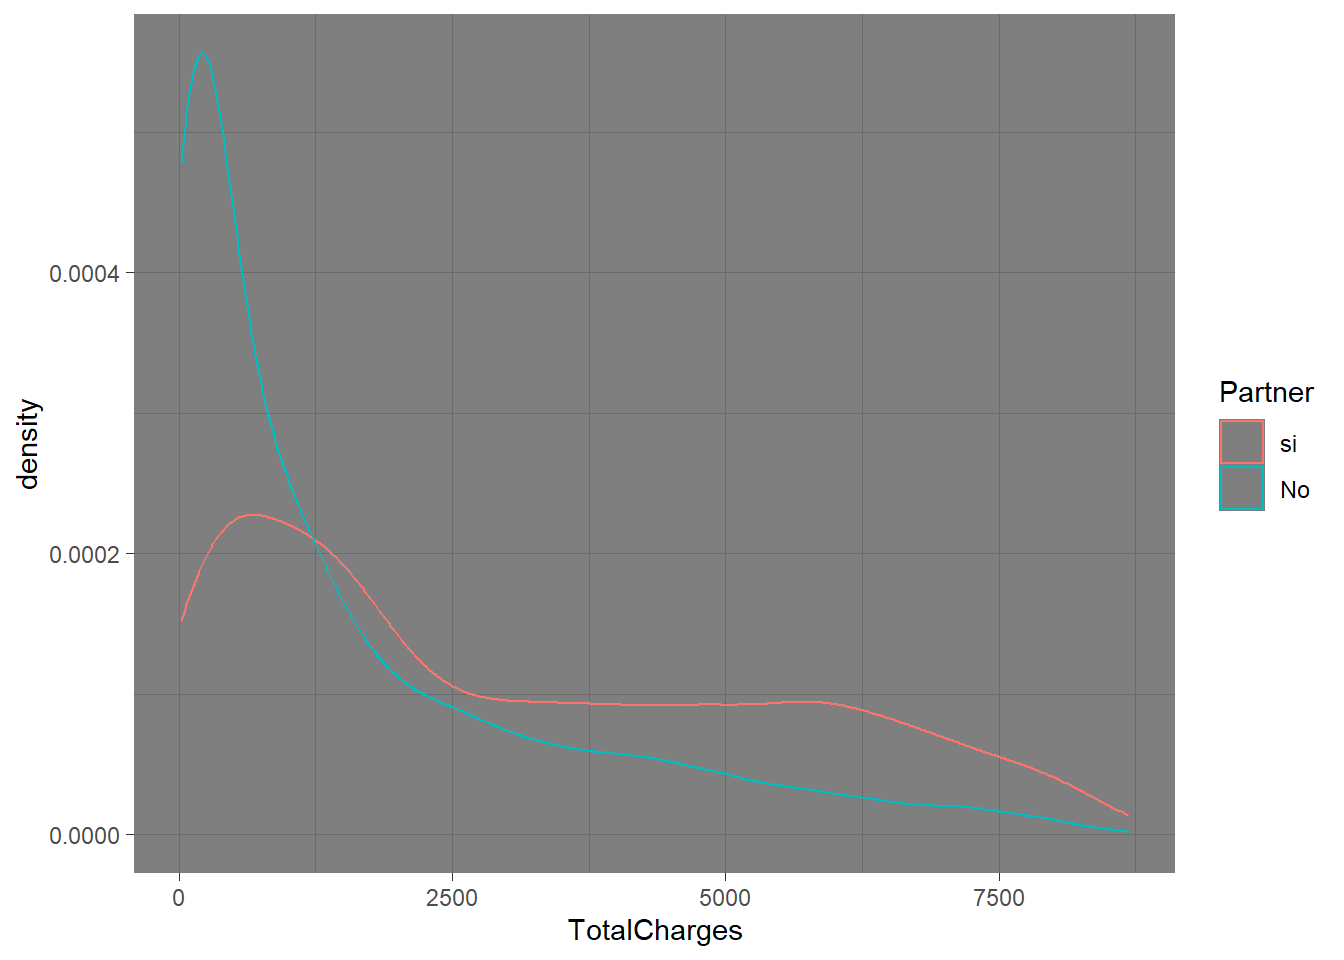
\includegraphics{model_Room_8_files/figure-latex/unnamed-chunk-6-1.pdf}

Existe una diferencia importante en los registros de dinero cobrado a
los clientes al considerar aquellos que tienen pareja. Al revisar el
gráfico anterior, se evidencia que las personas que informaron tener
pareja son las que presentan los cobros más altos. Esto se refleja en la
distribución, donde se observa una densidad mayor para valores altos en
comparación con las personas que declararon no tener pareja.

\hypertarget{balanceo-de-datos}{%
\subsubsection{Balanceo de datos}\label{balanceo-de-datos}}

\begin{Shaded}
\begin{Highlighting}[]
\NormalTok{data }\SpecialCharTok{\%\textgreater{}\%} 
  \FunctionTok{group\_by}\NormalTok{(Churn) }\SpecialCharTok{\%\textgreater{}\%} 
  \FunctionTok{count}\NormalTok{(}\AttributeTok{name =} \StringTok{"frec"}\NormalTok{) }\SpecialCharTok{\%\textgreater{}\%}
\FunctionTok{ungroup}\NormalTok{() }\SpecialCharTok{\%\textgreater{}\%}
\FunctionTok{mutate}\NormalTok{( }\AttributeTok{Porc=}\NormalTok{ frec}\SpecialCharTok{/}\FunctionTok{sum}\NormalTok{(frec))}
\end{Highlighting}
\end{Shaded}

\begin{verbatim}
## # A tibble: 2 x 3
##   Churn  frec  Porc
##   <fct> <int> <dbl>
## 1 si     1869 0.265
## 2 no     5174 0.735
\end{verbatim}

\begin{Shaded}
\begin{Highlighting}[]
\NormalTok{data }\SpecialCharTok{\%\textgreater{}\%}
\FunctionTok{group\_by}\NormalTok{(Churn) }\SpecialCharTok{\%\textgreater{}\%}
\FunctionTok{count}\NormalTok{( }\AttributeTok{name =} \StringTok{\textquotesingle{}frec\textquotesingle{}}\NormalTok{) }\SpecialCharTok{\%\textgreater{}\%}
\FunctionTok{ungroup}\NormalTok{() }\SpecialCharTok{\%\textgreater{}\%}
\FunctionTok{mutate}\NormalTok{( }\AttributeTok{Porc=}\NormalTok{ frec}\SpecialCharTok{/}\FunctionTok{sum}\NormalTok{(frec)) }\SpecialCharTok{\%\textgreater{}\%}
\FunctionTok{ggplot}\NormalTok{( }\FunctionTok{aes}\NormalTok{(}\AttributeTok{x=}\NormalTok{ Churn, }\AttributeTok{y=}\NormalTok{ Porc)) }\SpecialCharTok{+}
\FunctionTok{geom\_segment}\NormalTok{( }\FunctionTok{aes}\NormalTok{(}\AttributeTok{xend=}\NormalTok{ Churn, }\AttributeTok{y=}\DecValTok{0}\NormalTok{, }\AttributeTok{yend=}\NormalTok{Porc),}
\AttributeTok{color=} \StringTok{"steelblue"}\NormalTok{, }\AttributeTok{linewidth=} \DecValTok{1}\NormalTok{) }\SpecialCharTok{+}
\FunctionTok{geom\_point}\NormalTok{( }\AttributeTok{size=}\DecValTok{5}\NormalTok{, }\AttributeTok{color=} \StringTok{"steelblue"}\NormalTok{) }\SpecialCharTok{+}
\FunctionTok{coord\_flip}\NormalTok{() }\SpecialCharTok{+}
\FunctionTok{scale\_y\_continuous}\NormalTok{( }\AttributeTok{labels =} \FunctionTok{percent\_format}\NormalTok{()) }\SpecialCharTok{+}
\FunctionTok{labs}\NormalTok{(}\AttributeTok{title=} \StringTok{\textquotesingle{}Porcentaje de Clientes que Abandonan\textquotesingle{}}\NormalTok{,}
\AttributeTok{y=} \StringTok{"Porcentaje"}\NormalTok{, }\AttributeTok{x=} \StringTok{"Churn"}\NormalTok{) }\SpecialCharTok{+}
\FunctionTok{theme\_bw}\NormalTok{()}
\end{Highlighting}
\end{Shaded}

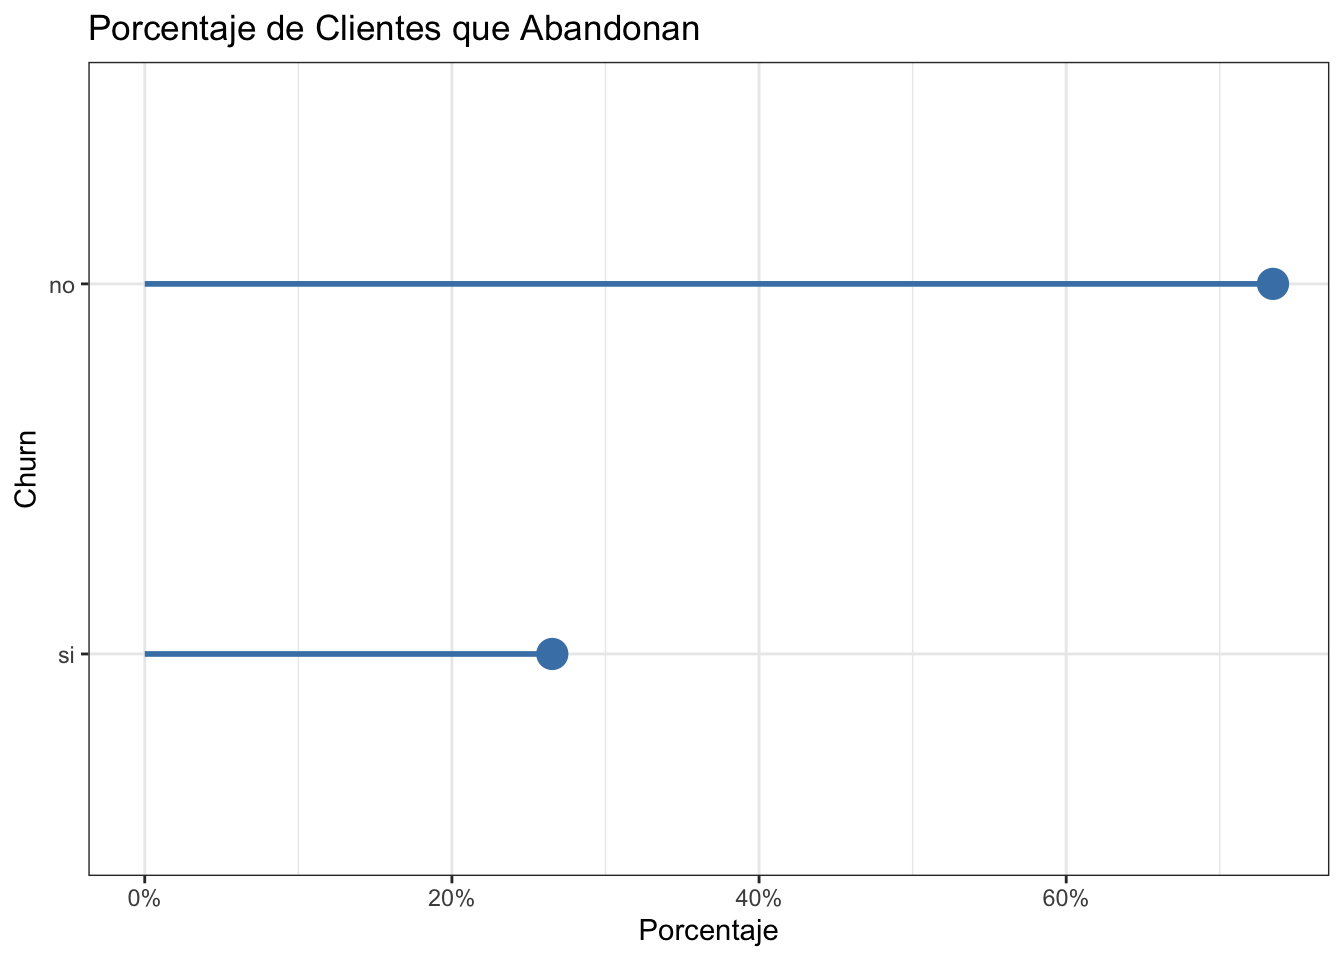
\includegraphics{model_Room_8_files/figure-latex/unnamed-chunk-7-1.pdf}

El porcentaje de clientes que abandonan el servicio de
telecomunicaciones es aproximadamente 3 a 1 en el muestra de análisis.

\hypertarget{eda-bivariado}{%
\subsubsection{EDA Bivariado}\label{eda-bivariado}}

\hypertarget{room-2}{%
\paragraph{Room 2}\label{room-2}}

\hypertarget{genero-vs-churn}{%
\subparagraph{Genero vs Churn}\label{genero-vs-churn}}

\textbf{Tabla}

\textbf{Grafico}

\textbf{Interpretacion}

\hypertarget{phoneservice-vs-churn}{%
\paragraph{PhoneService vs Churn}\label{phoneservice-vs-churn}}

\textbf{Interpretacion}

\hypertarget{room-4}{%
\paragraph{Room 4}\label{room-4}}

\hypertarget{seniorcitizen-vs-churn}{%
\subparagraph{SeniorCitizen vs Churn}\label{seniorcitizen-vs-churn}}

\textbf{Tabla}

\begin{Shaded}
\begin{Highlighting}[]
\NormalTok{data }\SpecialCharTok{\%\textgreater{}\%}
  \FunctionTok{group\_by}\NormalTok{(SeniorCitizen, Churn) }\SpecialCharTok{\%\textgreater{}\%}
  \FunctionTok{summarise}\NormalTok{(}
    \AttributeTok{N =} \FunctionTok{n}\NormalTok{(),}
    \AttributeTok{Porc =} \FunctionTok{round}\NormalTok{(}\DecValTok{100}\SpecialCharTok{*}\NormalTok{N}\SpecialCharTok{/}\FunctionTok{nrow}\NormalTok{(data),}\DecValTok{2}\NormalTok{)}
\NormalTok{  ) }\SpecialCharTok{\%\textgreater{}\%}
  \FunctionTok{mutate}\NormalTok{(}\AttributeTok{Porc\_grupo =} \FunctionTok{round}\NormalTok{(}\DecValTok{100}\SpecialCharTok{*}\NormalTok{N}\SpecialCharTok{/}\FunctionTok{sum}\NormalTok{(N),}\DecValTok{2}\NormalTok{)) }\OtherTok{{-}\textgreater{}}\NormalTok{ valores\_Sc}
\end{Highlighting}
\end{Shaded}

\begin{verbatim}
## `summarise()` has grouped output by 'SeniorCitizen'. You can override using the
## `.groups` argument.
\end{verbatim}

\begin{Shaded}
\begin{Highlighting}[]
\NormalTok{valores\_Sc}
\end{Highlighting}
\end{Shaded}

\begin{verbatim}
## # A tibble: 4 x 5
## # Groups:   SeniorCitizen [2]
##   SeniorCitizen Churn     N  Porc Porc_grupo
##   <fct>         <fct> <int> <dbl>      <dbl>
## 1 no            si     1393 19.8        23.6
## 2 no            no     4508 64.0        76.4
## 3 si            si      476  6.76       41.7
## 4 si            no      666  9.46       58.3
\end{verbatim}

\begin{Shaded}
\begin{Highlighting}[]
\CommentTok{\# Comentado por conflictos con paquete}
\CommentTok{\# tigerstats::rowPerc(xtabs(\textasciitilde{}SeniorCitizen+Churn, data=data) )}
\end{Highlighting}
\end{Shaded}

\textbf{Gráfico}

\begin{Shaded}
\begin{Highlighting}[]
\FunctionTok{ggplot}\NormalTok{(valores\_Sc, }\FunctionTok{aes}\NormalTok{(}\AttributeTok{x =}\NormalTok{ SeniorCitizen, }\AttributeTok{y =}\NormalTok{ Porc\_grupo, }\AttributeTok{fill =}\NormalTok{ Churn)) }\SpecialCharTok{+}
  \FunctionTok{geom\_col}\NormalTok{(}\AttributeTok{stat =} \StringTok{"identity"}\NormalTok{, }\AttributeTok{position =} \StringTok{"dodge"}\NormalTok{) }\SpecialCharTok{+}
  \FunctionTok{geom\_text}\NormalTok{(}\FunctionTok{aes}\NormalTok{(}\AttributeTok{label =}\NormalTok{ Porc\_grupo), }\AttributeTok{vjust =} \FloatTok{1.5}\NormalTok{,}
            \AttributeTok{position =} \FunctionTok{position\_dodge}\NormalTok{(.}\DecValTok{9}\NormalTok{))}
\end{Highlighting}
\end{Shaded}

\begin{verbatim}
## Warning in geom_col(stat = "identity", position = "dodge"): Ignoring unknown
## parameters: `stat`
\end{verbatim}

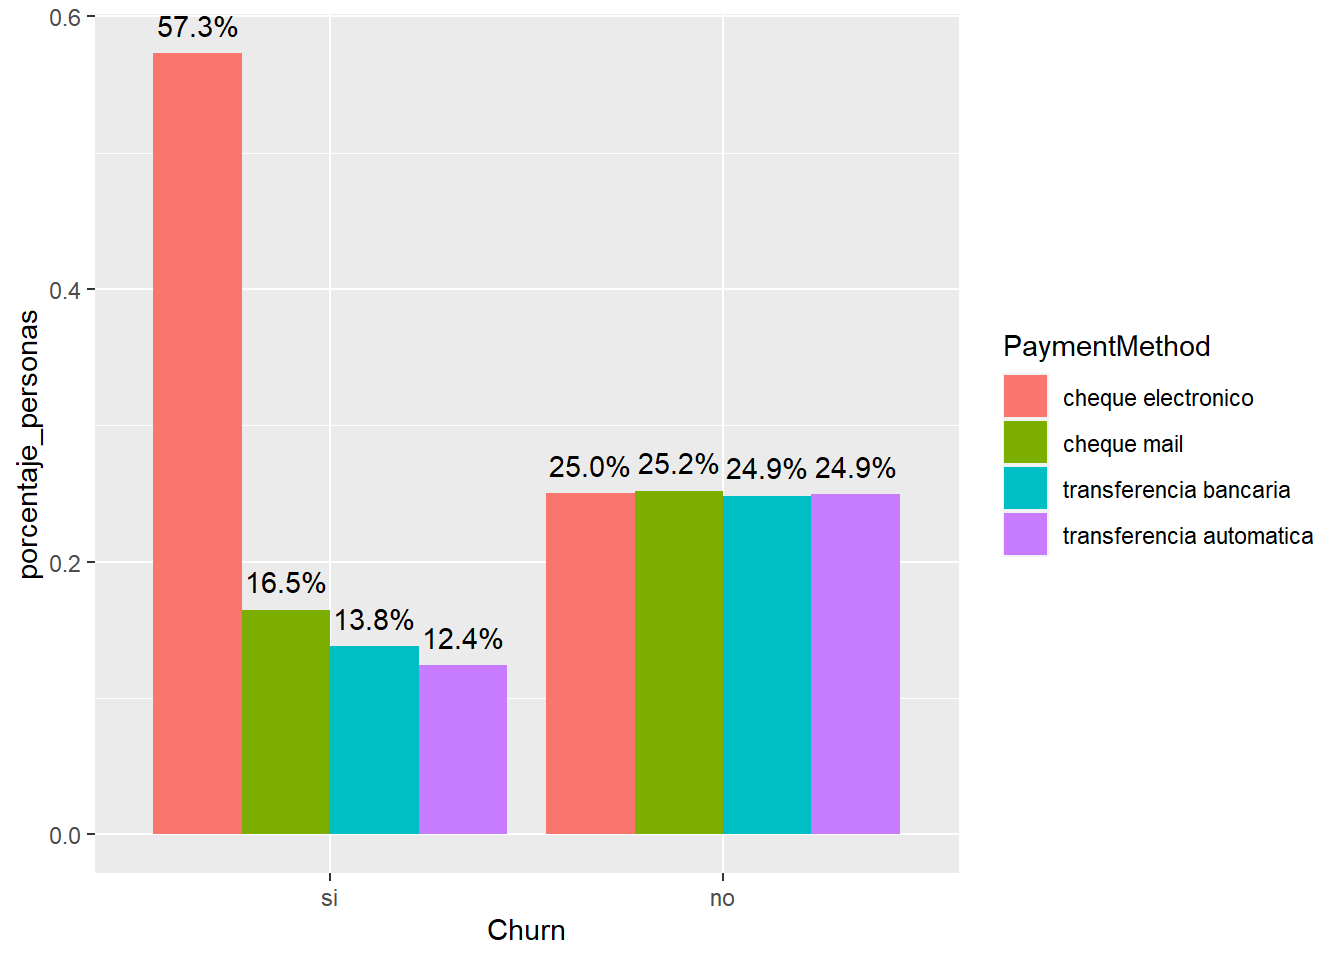
\includegraphics{model_Room_8_files/figure-latex/unnamed-chunk-13-1.pdf}

\textbf{Interpretación}

De los adultos mayores el 41\% abandonó el servicio, mientras que de los
no adultos mayores apenas un 24\% abandonó el servicio. Aparentemente,
un adulto mayor tiene mayor probabilidad de abandonar el servicio.

\hypertarget{multiplelines-vs-churn}{%
\subparagraph{MultipleLines vs Churn}\label{multiplelines-vs-churn}}

\textbf{Tabla}

\begin{Shaded}
\begin{Highlighting}[]
\NormalTok{data }\SpecialCharTok{\%\textgreater{}\%}
  \FunctionTok{group\_by}\NormalTok{(MultipleLines, Churn) }\SpecialCharTok{\%\textgreater{}\%}
  \FunctionTok{summarise}\NormalTok{(}
    \AttributeTok{N =} \FunctionTok{n}\NormalTok{(),}
    \AttributeTok{Porc =} \FunctionTok{round}\NormalTok{(}\DecValTok{100}\SpecialCharTok{*}\NormalTok{N}\SpecialCharTok{/}\FunctionTok{nrow}\NormalTok{(data),}\DecValTok{2}\NormalTok{)}
\NormalTok{  ) }\SpecialCharTok{\%\textgreater{}\%}
  \FunctionTok{mutate}\NormalTok{(}\AttributeTok{Porc\_grupo =} \FunctionTok{round}\NormalTok{(}\DecValTok{100}\SpecialCharTok{*}\NormalTok{N}\SpecialCharTok{/}\FunctionTok{sum}\NormalTok{(N),}\DecValTok{2}\NormalTok{)) }\OtherTok{{-}\textgreater{}}\NormalTok{ valores\_Ml}
\end{Highlighting}
\end{Shaded}

\begin{verbatim}
## `summarise()` has grouped output by 'MultipleLines'. You can override using the
## `.groups` argument.
\end{verbatim}

\begin{Shaded}
\begin{Highlighting}[]
\NormalTok{valores\_Ml}
\end{Highlighting}
\end{Shaded}

\begin{verbatim}
## # A tibble: 6 x 5
## # Groups:   MultipleLines [3]
##   MultipleLines Churn     N  Porc Porc_grupo
##   <fct>         <fct> <int> <dbl>      <dbl>
## 1 si            si      850 12.1        28.6
## 2 si            no     2121 30.1        71.4
## 3 no            si      849 12.0        25.0
## 4 no            no     2541 36.1        75.0
## 5 sin servicio  si      170  2.41       24.9
## 6 sin servicio  no      512  7.27       75.1
\end{verbatim}

\begin{Shaded}
\begin{Highlighting}[]
\CommentTok{\# Comentado por conflictos con paquete}
\CommentTok{\# tigerstats::rowPerc(xtabs(\textasciitilde{}MultipleLines+Churn, data=data) )}
\end{Highlighting}
\end{Shaded}

\textbf{Gráfico}

\begin{Shaded}
\begin{Highlighting}[]
\FunctionTok{ggplot}\NormalTok{(valores\_Ml, }\FunctionTok{aes}\NormalTok{(}\AttributeTok{x =}\NormalTok{ MultipleLines, }\AttributeTok{y =}\NormalTok{ N, }\AttributeTok{fill =}\NormalTok{ Churn)) }\SpecialCharTok{+}
  \FunctionTok{geom\_col}\NormalTok{(}\AttributeTok{stat =} \StringTok{"identity"}\NormalTok{, }\AttributeTok{position =} \StringTok{"dodge"}\NormalTok{) }\SpecialCharTok{+}
  \FunctionTok{geom\_text}\NormalTok{(}\FunctionTok{aes}\NormalTok{(}\AttributeTok{label =}\NormalTok{ N), }\AttributeTok{vjust =} \FloatTok{1.5}\NormalTok{,}
            \AttributeTok{position =} \FunctionTok{position\_dodge}\NormalTok{(.}\DecValTok{9}\NormalTok{))}
\end{Highlighting}
\end{Shaded}

\begin{verbatim}
## Warning in geom_col(stat = "identity", position = "dodge"): Ignoring unknown
## parameters: `stat`
\end{verbatim}

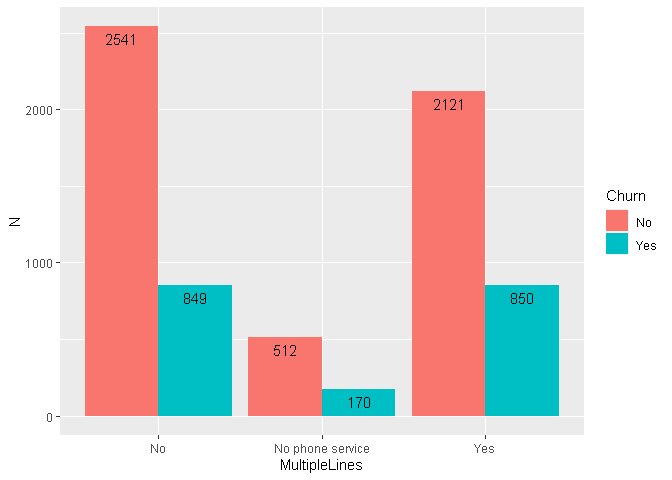
\includegraphics{model_Room_8_files/figure-latex/unnamed-chunk-16-1.pdf}

\textbf{Interpretación}

Entre las categorías de MultipleLines no hay mayor diferencia, entre los
que abandonan o no el servicio. Los porcentajes son muy parecidos.

\hypertarget{techsupport-vs-churn}{%
\subparagraph{TechSupport vs Churn}\label{techsupport-vs-churn}}

\begin{Shaded}
\begin{Highlighting}[]
\NormalTok{data }\SpecialCharTok{\%\textgreater{}\%}
  \FunctionTok{group\_by}\NormalTok{(TechSupport, Churn) }\SpecialCharTok{\%\textgreater{}\%}
  \FunctionTok{summarise}\NormalTok{(}
    \AttributeTok{N =} \FunctionTok{n}\NormalTok{(),}
    \AttributeTok{Porc =} \FunctionTok{round}\NormalTok{(}\DecValTok{100}\SpecialCharTok{*}\NormalTok{N}\SpecialCharTok{/}\FunctionTok{nrow}\NormalTok{(data),}\DecValTok{2}\NormalTok{)}
\NormalTok{  ) }\SpecialCharTok{\%\textgreater{}\%}
  \FunctionTok{mutate}\NormalTok{(}\AttributeTok{Porc\_grupo =} \FunctionTok{round}\NormalTok{(}\DecValTok{100}\SpecialCharTok{*}\NormalTok{N}\SpecialCharTok{/}\FunctionTok{sum}\NormalTok{(N),}\DecValTok{2}\NormalTok{)) }\OtherTok{{-}\textgreater{}}\NormalTok{ valores\_Ts}
\end{Highlighting}
\end{Shaded}

\begin{verbatim}
## `summarise()` has grouped output by 'TechSupport'. You can override using the
## `.groups` argument.
\end{verbatim}

\begin{Shaded}
\begin{Highlighting}[]
\NormalTok{valores\_Ts}
\end{Highlighting}
\end{Shaded}

\begin{verbatim}
## # A tibble: 6 x 5
## # Groups:   TechSupport [3]
##   TechSupport  Churn     N  Porc Porc_grupo
##   <fct>        <fct> <int> <dbl>      <dbl>
## 1 si           si      310   4.4       15.2
## 2 si           no     1734  24.6       84.8
## 3 no           si     1446  20.5       41.6
## 4 no           no     2027  28.8       58.4
## 5 sin servicio si      113   1.6        7.4
## 6 sin servicio no     1413  20.1       92.6
\end{verbatim}

\begin{Shaded}
\begin{Highlighting}[]
\CommentTok{\# Comentado por conflictos con paquete}
\CommentTok{\# tigerstats::rowPerc(xtabs(\textasciitilde{}TechSupport+Churn, data=data) )}
\end{Highlighting}
\end{Shaded}

\textbf{Gráfico}

\begin{Shaded}
\begin{Highlighting}[]
\FunctionTok{ggplot}\NormalTok{(valores\_Ts, }\FunctionTok{aes}\NormalTok{(}\AttributeTok{x =}\NormalTok{ TechSupport, }\AttributeTok{y =}\NormalTok{ N, }\AttributeTok{fill =}\NormalTok{ Churn)) }\SpecialCharTok{+}
  \FunctionTok{geom\_col}\NormalTok{(}\AttributeTok{stat =} \StringTok{"identity"}\NormalTok{, }\AttributeTok{position =} \StringTok{"dodge"}\NormalTok{) }\SpecialCharTok{+}
  \FunctionTok{geom\_text}\NormalTok{(}\FunctionTok{aes}\NormalTok{(}\AttributeTok{label =}\NormalTok{ N), }\AttributeTok{vjust =} \FloatTok{1.5}\NormalTok{,}
            \AttributeTok{position =} \FunctionTok{position\_dodge}\NormalTok{(.}\DecValTok{9}\NormalTok{))}
\end{Highlighting}
\end{Shaded}

\begin{verbatim}
## Warning in geom_col(stat = "identity", position = "dodge"): Ignoring unknown
## parameters: `stat`
\end{verbatim}

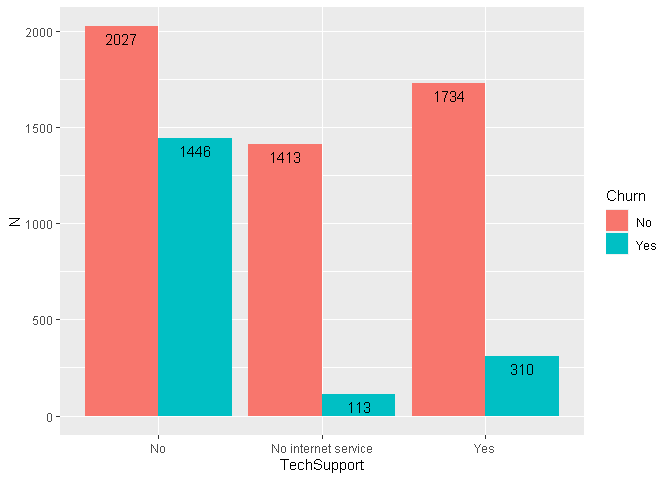
\includegraphics{model_Room_8_files/figure-latex/unnamed-chunk-19-1.pdf}

\textbf{Interpretación}

Los que no cuentan con soporte técnico, el 41.68\% abandona el servicio.
Por otro lado, los que si cuentan con soporte apenas un 15.17\% abandona
el servicio y los que no tienen internet contratado solo un 7.40\%
abandona el servicio.

\hypertarget{paymentmethod-vs-churn}{%
\subparagraph{PaymentMethod vs Churn}\label{paymentmethod-vs-churn}}

\begin{Shaded}
\begin{Highlighting}[]
\NormalTok{data }\SpecialCharTok{\%\textgreater{}\%}
  \FunctionTok{group\_by}\NormalTok{(PaymentMethod, Churn) }\SpecialCharTok{\%\textgreater{}\%}
  \FunctionTok{summarise}\NormalTok{(}
    \AttributeTok{N =} \FunctionTok{n}\NormalTok{(),}
    \AttributeTok{Porc =} \FunctionTok{round}\NormalTok{(}\DecValTok{100}\SpecialCharTok{*}\NormalTok{N}\SpecialCharTok{/}\FunctionTok{nrow}\NormalTok{(data),}\DecValTok{2}\NormalTok{)}
\NormalTok{  ) }\SpecialCharTok{\%\textgreater{}\%}
  \FunctionTok{mutate}\NormalTok{(}\AttributeTok{Porc\_grupo =} \FunctionTok{round}\NormalTok{(}\DecValTok{100}\SpecialCharTok{*}\NormalTok{N}\SpecialCharTok{/}\FunctionTok{sum}\NormalTok{(N),}\DecValTok{2}\NormalTok{)) }\OtherTok{{-}\textgreater{}}\NormalTok{ valores\_Pm}
\end{Highlighting}
\end{Shaded}

\begin{verbatim}
## `summarise()` has grouped output by 'PaymentMethod'. You can override using the
## `.groups` argument.
\end{verbatim}

\begin{Shaded}
\begin{Highlighting}[]
\NormalTok{valores\_Pm}
\end{Highlighting}
\end{Shaded}

\begin{verbatim}
## # A tibble: 8 x 5
## # Groups:   PaymentMethod [4]
##   PaymentMethod            Churn     N  Porc Porc_grupo
##   <fct>                    <fct> <int> <dbl>      <dbl>
## 1 cheque electronico       si     1071 15.2        45.3
## 2 cheque electronico       no     1294 18.4        54.7
## 3 cheque mail              si      308  4.37       19.1
## 4 cheque mail              no     1304 18.5        80.9
## 5 transferencia bancaria   si      258  3.66       16.7
## 6 transferencia bancaria   no     1286 18.3        83.3
## 7 transferencia automatica si      232  3.29       15.2
## 8 transferencia automatica no     1290 18.3        84.8
\end{verbatim}

\begin{Shaded}
\begin{Highlighting}[]
\CommentTok{\# Comentado por conflictos con paquete}
\CommentTok{\# tigerstats::rowPerc(xtabs(\textasciitilde{}PaymentMethod+Churn, data=data) )}
\end{Highlighting}
\end{Shaded}

\textbf{Gráfico}

\begin{Shaded}
\begin{Highlighting}[]
\FunctionTok{ggplot}\NormalTok{(valores\_Pm, }\FunctionTok{aes}\NormalTok{(}\AttributeTok{x =}\NormalTok{ PaymentMethod, }\AttributeTok{y =}\NormalTok{ N, }\AttributeTok{fill =}\NormalTok{ Churn)) }\SpecialCharTok{+}
  \FunctionTok{geom\_col}\NormalTok{(}\AttributeTok{stat =} \StringTok{"identity"}\NormalTok{, }\AttributeTok{position =} \StringTok{"dodge"}\NormalTok{) }\SpecialCharTok{+}
  \FunctionTok{geom\_text}\NormalTok{(}\FunctionTok{aes}\NormalTok{(}\AttributeTok{label =}\NormalTok{ N), }\AttributeTok{vjust =} \FloatTok{1.5}\NormalTok{,}
            \AttributeTok{position =} \FunctionTok{position\_dodge}\NormalTok{(.}\DecValTok{9}\NormalTok{))}
\end{Highlighting}
\end{Shaded}

\begin{verbatim}
## Warning in geom_col(stat = "identity", position = "dodge"): Ignoring unknown
## parameters: `stat`
\end{verbatim}

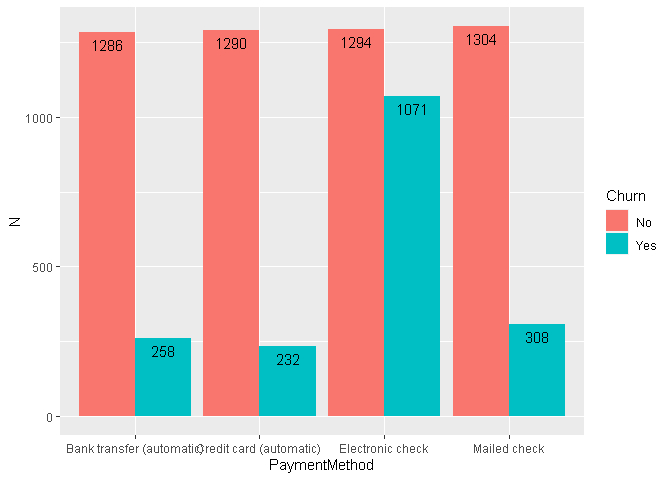
\includegraphics{model_Room_8_files/figure-latex/unnamed-chunk-22-1.pdf}

\textbf{Interpretación}

A excepción de los que pagan con cheque electrónico los porcentajes de
abandono son muy parecidos. En el caso de los que pagan con cheque
electrónico un 45.29\% abandona el servicio.

\hypertarget{eda-multivariado}{%
\subsubsection{EDA Multivariado}\label{eda-multivariado}}

\hypertarget{monthlycharges-vs-paymentmethod-vs-churn}{%
\paragraph{MonthlyCharges vs PaymentMethod vs
Churn}\label{monthlycharges-vs-paymentmethod-vs-churn}}

\textbf{Gráfico 1}

\begin{Shaded}
\begin{Highlighting}[]
\FunctionTok{ggplot}\NormalTok{(data, }\FunctionTok{aes}\NormalTok{(}\AttributeTok{x =}\NormalTok{ PaymentMethod, }\AttributeTok{y =}\NormalTok{ MonthlyCharges, }\AttributeTok{fill =}\NormalTok{ Churn)) }\SpecialCharTok{+}
  \FunctionTok{geom\_boxplot}\NormalTok{()}
\end{Highlighting}
\end{Shaded}

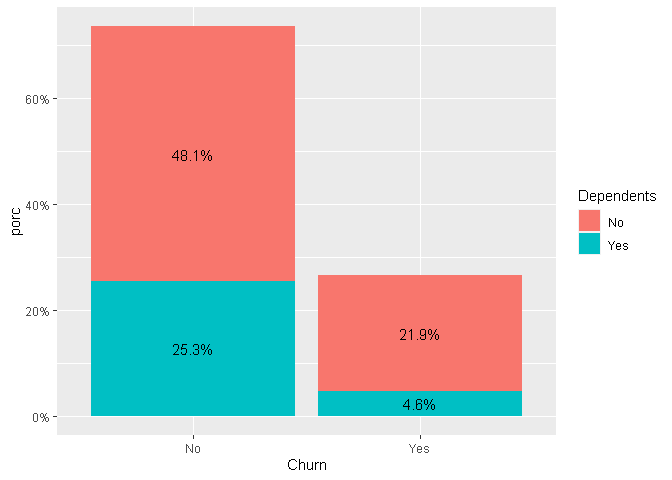
\includegraphics{model_Room_8_files/figure-latex/unnamed-chunk-23-1.pdf}

\textbf{Interpretación}

\textbf{Gráfico 2}

\begin{Shaded}
\begin{Highlighting}[]
\FunctionTok{ggplot}\NormalTok{(data, }\FunctionTok{aes}\NormalTok{(}\AttributeTok{x =}\NormalTok{ Churn, }\AttributeTok{y =}\NormalTok{ MonthlyCharges, }\AttributeTok{fill =}\NormalTok{ PaymentMethod)) }\SpecialCharTok{+}
  \FunctionTok{geom\_boxplot}\NormalTok{()}
\end{Highlighting}
\end{Shaded}

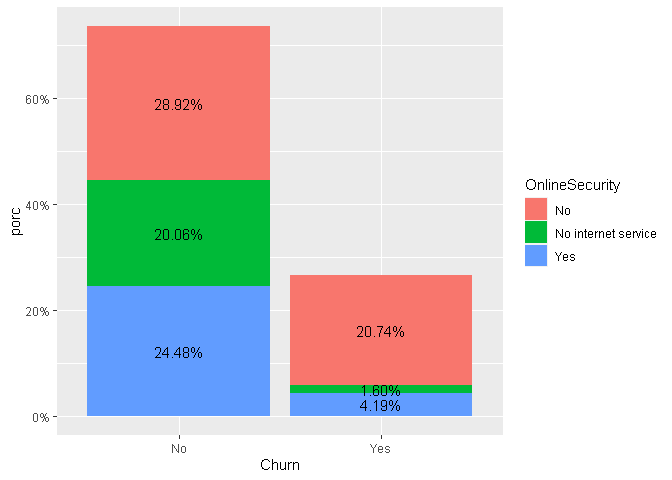
\includegraphics{model_Room_8_files/figure-latex/unnamed-chunk-24-1.pdf}

\textbf{Interpretación}

Los montos de pago de aquellos que abandonan el servicio son superiores
a aquellos que permanecen con excepción de los que pagan por cheque
electrónico.

\hypertarget{room-6}{%
\subsubsection{Room 6}\label{room-6}}

\hypertarget{room-7}{%
\subsubsection{Room 7}\label{room-7}}

\hypertarget{room-8}{%
\subsubsection{Room 8}\label{room-8}}

\hypertarget{eda-bivariado-entre-churn-y-dependents}{%
\paragraph{Eda Bivariado entre churn y
Dependents}\label{eda-bivariado-entre-churn-y-dependents}}

\begin{Shaded}
\begin{Highlighting}[]
\NormalTok{data }\SpecialCharTok{\%\textgreater{}\%} \FunctionTok{tabyl}\NormalTok{(Churn, Dependents ) }\OtherTok{{-}\textgreater{}}\NormalTok{ t1}

\NormalTok{t1 }\SpecialCharTok{\%\textgreater{}\%} \FunctionTok{adorn\_totals}\NormalTok{(}\FunctionTok{c}\NormalTok{(}\StringTok{"row"}\NormalTok{, }\StringTok{"col"}\NormalTok{)) }\SpecialCharTok{\%\textgreater{}\%} \FunctionTok{adorn\_percentages}\NormalTok{(}\StringTok{"all"}\NormalTok{) }\SpecialCharTok{\%\textgreater{}\%}
\FunctionTok{adorn\_pct\_formatting}\NormalTok{(}\AttributeTok{rounding =} \StringTok{"half up"}\NormalTok{, }\AttributeTok{digits =} \DecValTok{0}\NormalTok{) }\SpecialCharTok{\%\textgreater{}\%} \FunctionTok{adorn\_ns}\NormalTok{() }\SpecialCharTok{\%\textgreater{}\%}
  \FunctionTok{adorn\_title}\NormalTok{(}\StringTok{"combined"}\NormalTok{) }\SpecialCharTok{\%\textgreater{}\%}\NormalTok{ knitr}\SpecialCharTok{::}\FunctionTok{kable}\NormalTok{()}
\end{Highlighting}
\end{Shaded}

\begin{longtable}[]{@{}llll@{}}
\toprule\noalign{}
Churn/Dependents & si & No & Total \\
\midrule\noalign{}
\endhead
\bottomrule\noalign{}
\endlastfoot
si & 5\% (326) & 22\% (1,543) & 27\% (1,869) \\
no & 25\% (1,784) & 48\% (3,390) & 73\% (5,174) \\
Total & 30\% (2,110) & 70\% (4,933) & 100\% (7,043) \\
\end{longtable}

\begin{Shaded}
\begin{Highlighting}[]
\NormalTok{data }\SpecialCharTok{\%\textgreater{}\%} \FunctionTok{count}\NormalTok{(Churn, Dependents) }\SpecialCharTok{\%\textgreater{}\%}
  \FunctionTok{mutate}\NormalTok{(}\AttributeTok{porc =}\NormalTok{ n }\SpecialCharTok{/} \FunctionTok{sum}\NormalTok{(n)) }\SpecialCharTok{\%\textgreater{}\%} 
  \FunctionTok{ggplot}\NormalTok{(}\FunctionTok{aes}\NormalTok{(}\AttributeTok{fill=}\NormalTok{Dependents, }\AttributeTok{y=}\NormalTok{porc, }\AttributeTok{x=}\NormalTok{Churn)) }\SpecialCharTok{+} 
    \FunctionTok{geom\_col}\NormalTok{(}\AttributeTok{position=}\StringTok{"stack"}\NormalTok{) }\SpecialCharTok{+}
    \FunctionTok{geom\_text}\NormalTok{(}\FunctionTok{aes}\NormalTok{(}\AttributeTok{label=}\NormalTok{scales}\SpecialCharTok{::}\FunctionTok{percent}\NormalTok{(porc)),}\AttributeTok{position =} \FunctionTok{position\_stack}\NormalTok{(}\AttributeTok{vjust=}\FloatTok{0.5}\NormalTok{))}\SpecialCharTok{+}
  \FunctionTok{scale\_y\_continuous}\NormalTok{(}\AttributeTok{labels =}\NormalTok{ scales}\SpecialCharTok{::}\FunctionTok{percent\_format}\NormalTok{()) }
\end{Highlighting}
\end{Shaded}

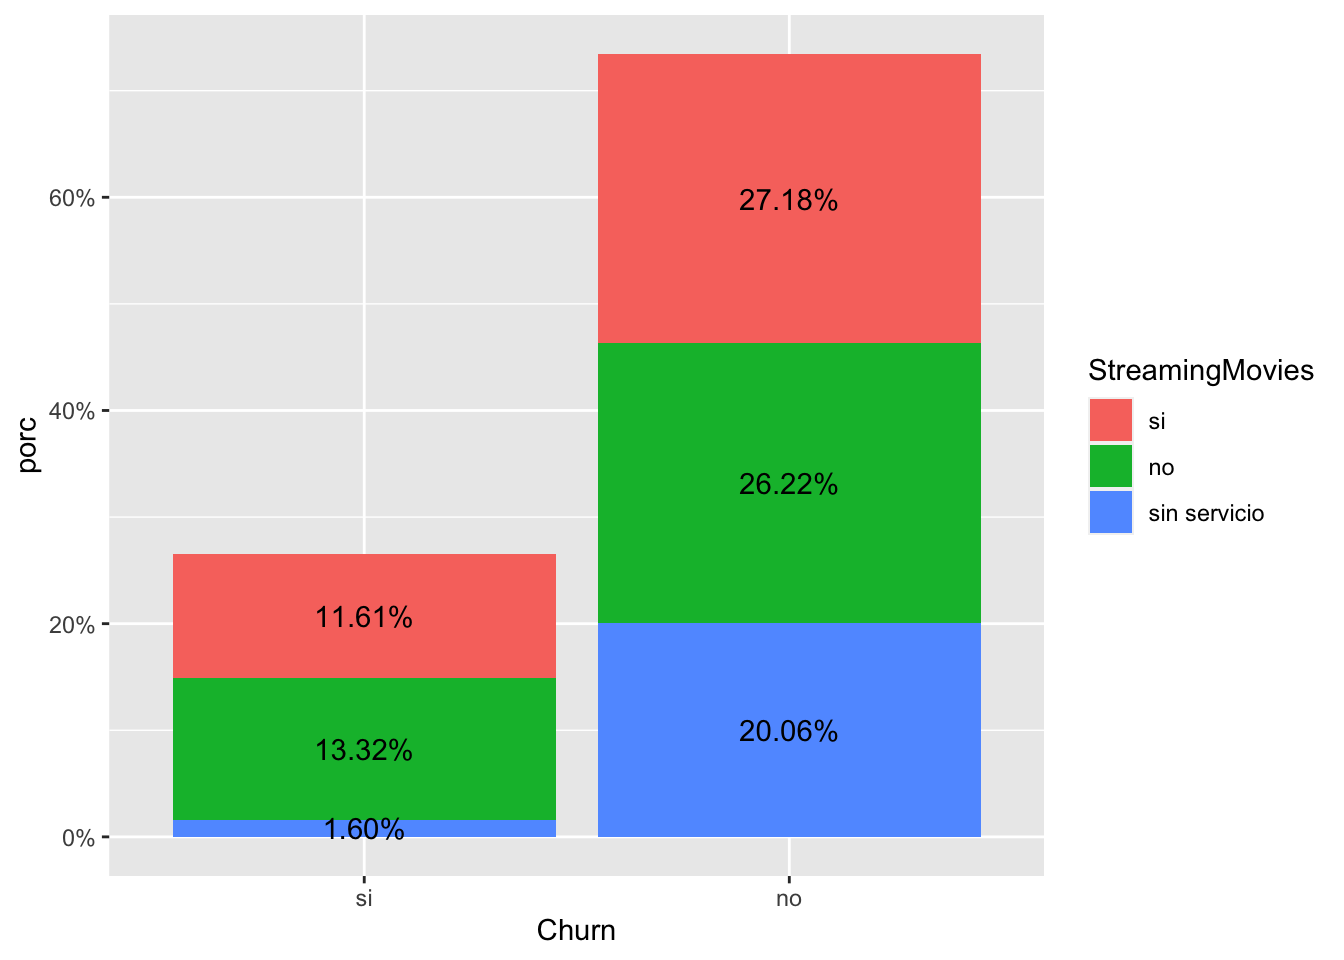
\includegraphics{model_Room_8_files/figure-latex/unnamed-chunk-25-1.pdf}

De la muestra analizada alrededor del 27\% corresponde a individuos que
dejaron sus planes en el último mes. Además se conoce que el 4,6\% de
estos individuos contaban con personas dependientes.

\hypertarget{eda-bivariado-entre-churn-y-onlinesecurity}{%
\paragraph{Eda Bivariado entre churn y
OnlineSecurity}\label{eda-bivariado-entre-churn-y-onlinesecurity}}

\begin{Shaded}
\begin{Highlighting}[]
\NormalTok{data }\SpecialCharTok{\%\textgreater{}\%} \FunctionTok{tabyl}\NormalTok{(Churn,OnlineSecurity ) }\OtherTok{{-}\textgreater{}}\NormalTok{ t2}

\NormalTok{t2 }\SpecialCharTok{\%\textgreater{}\%} \FunctionTok{adorn\_totals}\NormalTok{(}\FunctionTok{c}\NormalTok{(}\StringTok{"row"}\NormalTok{, }\StringTok{"col"}\NormalTok{)) }\SpecialCharTok{\%\textgreater{}\%} \FunctionTok{adorn\_percentages}\NormalTok{(}\StringTok{"all"}\NormalTok{) }\SpecialCharTok{\%\textgreater{}\%}
\FunctionTok{adorn\_pct\_formatting}\NormalTok{(}\AttributeTok{rounding =} \StringTok{"half up"}\NormalTok{, }\AttributeTok{digits =} \DecValTok{0}\NormalTok{) }\SpecialCharTok{\%\textgreater{}\%} \FunctionTok{adorn\_ns}\NormalTok{()}\SpecialCharTok{\%\textgreater{}\%} \FunctionTok{adorn\_title}\NormalTok{(}\StringTok{"combined"}\NormalTok{)}\SpecialCharTok{\%\textgreater{}\%}\NormalTok{ knitr}\SpecialCharTok{::}\FunctionTok{kable}\NormalTok{()}
\end{Highlighting}
\end{Shaded}

\begin{longtable}[]{@{}
  >{\raggedright\arraybackslash}p{(\columnwidth - 8\tabcolsep) * \real{0.2958}}
  >{\raggedright\arraybackslash}p{(\columnwidth - 8\tabcolsep) * \real{0.1690}}
  >{\raggedright\arraybackslash}p{(\columnwidth - 8\tabcolsep) * \real{0.1690}}
  >{\raggedright\arraybackslash}p{(\columnwidth - 8\tabcolsep) * \real{0.1831}}
  >{\raggedright\arraybackslash}p{(\columnwidth - 8\tabcolsep) * \real{0.1831}}@{}}
\toprule\noalign{}
\begin{minipage}[b]{\linewidth}\raggedright
Churn/OnlineSecurity
\end{minipage} & \begin{minipage}[b]{\linewidth}\raggedright
No
\end{minipage} & \begin{minipage}[b]{\linewidth}\raggedright
Yes
\end{minipage} & \begin{minipage}[b]{\linewidth}\raggedright
sin servicio
\end{minipage} & \begin{minipage}[b]{\linewidth}\raggedright
Total
\end{minipage} \\
\midrule\noalign{}
\endhead
\bottomrule\noalign{}
\endlastfoot
si & 21\% (1,461) & 4\% (295) & 2\% (113) & 27\% (1,869) \\
no & 29\% (2,037) & 24\% (1,724) & 20\% (1,413) & 73\% (5,174) \\
Total & 50\% (3,498) & 29\% (2,019) & 22\% (1,526) & 100\% (7,043) \\
\end{longtable}

\begin{Shaded}
\begin{Highlighting}[]
\NormalTok{data }\SpecialCharTok{\%\textgreater{}\%} \FunctionTok{count}\NormalTok{(Churn, OnlineSecurity) }\SpecialCharTok{\%\textgreater{}\%}
  \FunctionTok{mutate}\NormalTok{(}\AttributeTok{porc =}\NormalTok{ n }\SpecialCharTok{/} \FunctionTok{sum}\NormalTok{(n)) }\SpecialCharTok{\%\textgreater{}\%} 
  \FunctionTok{ggplot}\NormalTok{(}\FunctionTok{aes}\NormalTok{(}\AttributeTok{fill=}\NormalTok{OnlineSecurity, }\AttributeTok{y=}\NormalTok{porc, }\AttributeTok{x=}\NormalTok{Churn)) }\SpecialCharTok{+} 
    \FunctionTok{geom\_col}\NormalTok{(}\AttributeTok{position=}\StringTok{"stack"}\NormalTok{) }\SpecialCharTok{+}
    \FunctionTok{geom\_text}\NormalTok{(}\FunctionTok{aes}\NormalTok{(}\AttributeTok{label=}\NormalTok{scales}\SpecialCharTok{::}\FunctionTok{percent}\NormalTok{(porc)),}\AttributeTok{position =} \FunctionTok{position\_stack}\NormalTok{(}\AttributeTok{vjust=}\FloatTok{0.5}\NormalTok{))}\SpecialCharTok{+}
  \FunctionTok{scale\_y\_continuous}\NormalTok{(}\AttributeTok{labels =}\NormalTok{ scales}\SpecialCharTok{::}\FunctionTok{percent\_format}\NormalTok{()) }
\end{Highlighting}
\end{Shaded}

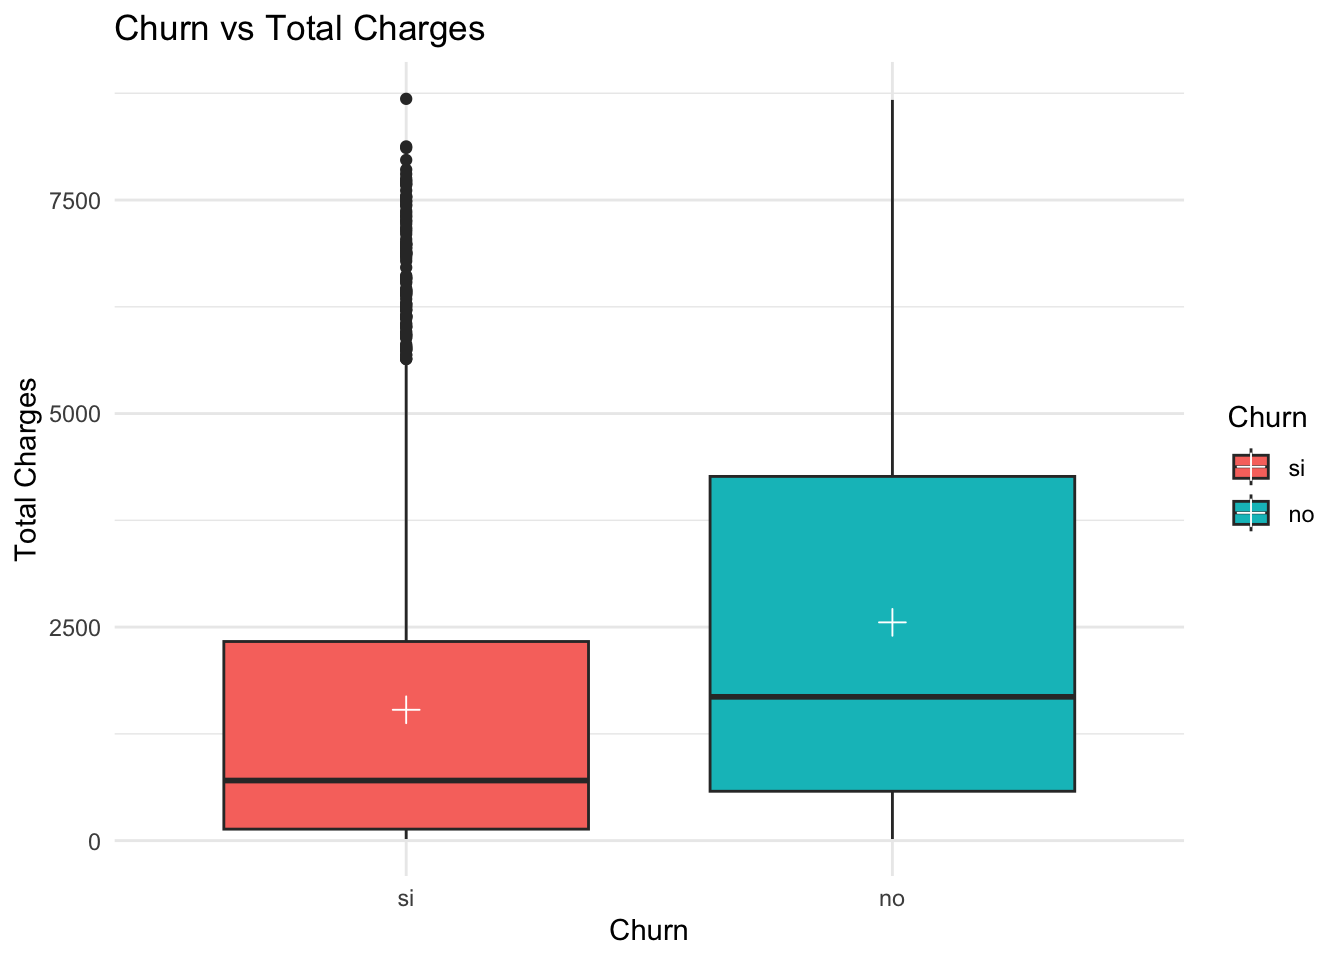
\includegraphics{model_Room_8_files/figure-latex/unnamed-chunk-26-1.pdf}

El 20,74\% de los indviduos analizados y que abandonaron el servicio no
contaban con seguridad en línea. Por otro lado aquellos que no salieron
del plan reflejaron una participación similar con relación al servicio
de seguridad en línea.

\hypertarget{eda-bivariado-entre-churn-y-streamingmovies}{%
\paragraph{Eda Bivariado entre Churn y
StreamingMovies}\label{eda-bivariado-entre-churn-y-streamingmovies}}

\begin{Shaded}
\begin{Highlighting}[]
\NormalTok{data }\SpecialCharTok{\%\textgreater{}\%} \FunctionTok{tabyl}\NormalTok{(Churn,StreamingMovies) }\OtherTok{{-}\textgreater{}}\NormalTok{ t3}

\NormalTok{t3 }\SpecialCharTok{\%\textgreater{}\%} \FunctionTok{adorn\_totals}\NormalTok{(}\FunctionTok{c}\NormalTok{(}\StringTok{"row"}\NormalTok{, }\StringTok{"col"}\NormalTok{)) }\SpecialCharTok{\%\textgreater{}\%} \FunctionTok{adorn\_percentages}\NormalTok{(}\StringTok{"all"}\NormalTok{) }\SpecialCharTok{\%\textgreater{}\%}
\FunctionTok{adorn\_pct\_formatting}\NormalTok{(}\AttributeTok{rounding =} \StringTok{"half up"}\NormalTok{, }\AttributeTok{digits =} \DecValTok{0}\NormalTok{) }\SpecialCharTok{\%\textgreater{}\%} \FunctionTok{adorn\_ns}\NormalTok{()}\SpecialCharTok{\%\textgreater{}\%} \FunctionTok{adorn\_title}\NormalTok{(}\StringTok{"combined"}\NormalTok{)}\SpecialCharTok{\%\textgreater{}\%}\NormalTok{ knitr}\SpecialCharTok{::}\FunctionTok{kable}\NormalTok{()}
\end{Highlighting}
\end{Shaded}

\begin{longtable}[]{@{}
  >{\raggedright\arraybackslash}p{(\columnwidth - 8\tabcolsep) * \real{0.3056}}
  >{\raggedright\arraybackslash}p{(\columnwidth - 8\tabcolsep) * \real{0.1667}}
  >{\raggedright\arraybackslash}p{(\columnwidth - 8\tabcolsep) * \real{0.1667}}
  >{\raggedright\arraybackslash}p{(\columnwidth - 8\tabcolsep) * \real{0.1806}}
  >{\raggedright\arraybackslash}p{(\columnwidth - 8\tabcolsep) * \real{0.1806}}@{}}
\toprule\noalign{}
\begin{minipage}[b]{\linewidth}\raggedright
Churn/StreamingMovies
\end{minipage} & \begin{minipage}[b]{\linewidth}\raggedright
si
\end{minipage} & \begin{minipage}[b]{\linewidth}\raggedright
no
\end{minipage} & \begin{minipage}[b]{\linewidth}\raggedright
sin servicio
\end{minipage} & \begin{minipage}[b]{\linewidth}\raggedright
Total
\end{minipage} \\
\midrule\noalign{}
\endhead
\bottomrule\noalign{}
\endlastfoot
si & 12\% (818) & 13\% (938) & 2\% (113) & 27\% (1,869) \\
no & 27\% (1,914) & 26\% (1,847) & 20\% (1,413) & 73\% (5,174) \\
Total & 39\% (2,732) & 40\% (2,785) & 22\% (1,526) & 100\% (7,043) \\
\end{longtable}

\begin{Shaded}
\begin{Highlighting}[]
\NormalTok{data }\SpecialCharTok{\%\textgreater{}\%} \FunctionTok{count}\NormalTok{(Churn, StreamingMovies) }\SpecialCharTok{\%\textgreater{}\%}
  \FunctionTok{mutate}\NormalTok{(}\AttributeTok{porc =}\NormalTok{ n }\SpecialCharTok{/} \FunctionTok{sum}\NormalTok{(n)) }\SpecialCharTok{\%\textgreater{}\%} 
  \FunctionTok{ggplot}\NormalTok{(}\FunctionTok{aes}\NormalTok{(}\AttributeTok{fill=}\NormalTok{StreamingMovies, }\AttributeTok{y=}\NormalTok{porc, }\AttributeTok{x=}\NormalTok{Churn)) }\SpecialCharTok{+} 
    \FunctionTok{geom\_col}\NormalTok{(}\AttributeTok{position=}\StringTok{"stack"}\NormalTok{) }\SpecialCharTok{+}
    \FunctionTok{geom\_text}\NormalTok{(}\FunctionTok{aes}\NormalTok{(}\AttributeTok{label=}\NormalTok{scales}\SpecialCharTok{::}\FunctionTok{percent}\NormalTok{(porc)),}\AttributeTok{position =} \FunctionTok{position\_stack}\NormalTok{(}\AttributeTok{vjust=}\FloatTok{0.5}\NormalTok{))}\SpecialCharTok{+}
  \FunctionTok{scale\_y\_continuous}\NormalTok{(}\AttributeTok{labels =}\NormalTok{ scales}\SpecialCharTok{::}\FunctionTok{percent\_format}\NormalTok{()) }
\end{Highlighting}
\end{Shaded}

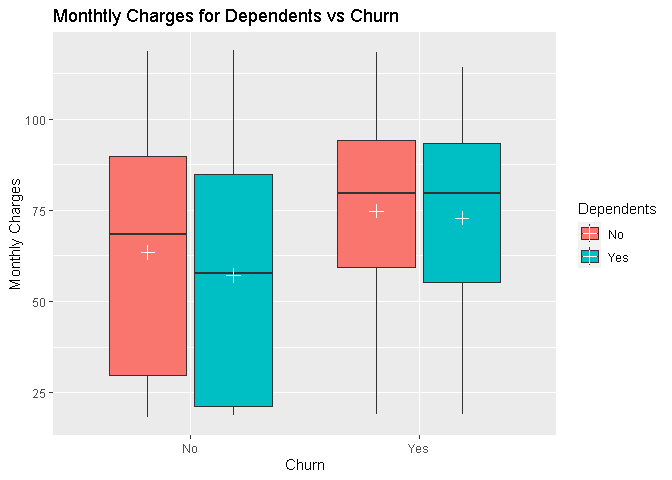
\includegraphics{model_Room_8_files/figure-latex/unnamed-chunk-27-1.pdf}

El 13,32\% de los indviduos analizados y que abandonaron el servicio no
contaban con servicio de Streaming Movies. Sin embargo, tanto para el
grupo que abandonaron o mantuvieron el servicio no se evidencia una
importancia relevante para su salidad del plan.

\hypertarget{eda-bivariado-entre-churn-y-total-charges}{%
\paragraph{Eda Bivariado entre churn y Total
Charges}\label{eda-bivariado-entre-churn-y-total-charges}}

\begin{Shaded}
\begin{Highlighting}[]
\NormalTok{data }\SpecialCharTok{\%\textgreater{}\%}  \FunctionTok{group\_by}\NormalTok{(Churn) }\SpecialCharTok{\%\textgreater{}\%} 
  \FunctionTok{summarise}\NormalTok{(}\AttributeTok{n =} \FunctionTok{n}\NormalTok{(),}
            \AttributeTok{promedio =} \FunctionTok{mean}\NormalTok{(TotalCharges,}\AttributeTok{na.rm =}\NormalTok{ T),}
            \AttributeTok{n\_missing =} \FunctionTok{sum}\NormalTok{(}\FunctionTok{is.na}\NormalTok{(TotalCharges)),}
            \AttributeTok{desv =} \FunctionTok{sd}\NormalTok{(TotalCharges, }\AttributeTok{na.rm =}\NormalTok{T)) }\OtherTok{{-}\textgreater{}}\NormalTok{ t4}
\NormalTok{t4}
\end{Highlighting}
\end{Shaded}

\begin{verbatim}
## # A tibble: 2 x 5
##   Churn     n promedio n_missing  desv
##   <fct> <int>    <dbl>     <int> <dbl>
## 1 si     1869    1532.         0 1891.
## 2 no     5174    2555.        11 2329.
\end{verbatim}

\begin{Shaded}
\begin{Highlighting}[]
\NormalTok{data }\SpecialCharTok{\%\textgreater{}\%}
  \FunctionTok{ggplot}\NormalTok{(}\FunctionTok{aes}\NormalTok{(}\AttributeTok{x =}\NormalTok{ Churn, }\AttributeTok{y =}\NormalTok{ TotalCharges, }\AttributeTok{fill =}\NormalTok{ Churn)) }\SpecialCharTok{+}
  \FunctionTok{geom\_boxplot}\NormalTok{() }\SpecialCharTok{+}
  \FunctionTok{stat\_summary}\NormalTok{(}\AttributeTok{fun =}\NormalTok{ mean, }\AttributeTok{geom =} \StringTok{"point"}\NormalTok{, }\AttributeTok{shape =} \DecValTok{3}\NormalTok{, }\AttributeTok{size =} \DecValTok{3}\NormalTok{,}
               \AttributeTok{color =} \StringTok{"white"}\NormalTok{, }\AttributeTok{position =} \FunctionTok{position\_dodge}\NormalTok{(}\AttributeTok{width =} \FloatTok{0.75}\NormalTok{)) }\SpecialCharTok{+}
  \FunctionTok{labs}\NormalTok{(}\AttributeTok{title =} \StringTok{"Churn vs Total Charges"}\NormalTok{,}
       \AttributeTok{x =} \StringTok{"Churn"}\NormalTok{,}
       \AttributeTok{y =} \StringTok{"Total Charges"}\NormalTok{) }\SpecialCharTok{+}
        \FunctionTok{theme\_minimal}\NormalTok{()}
\end{Highlighting}
\end{Shaded}

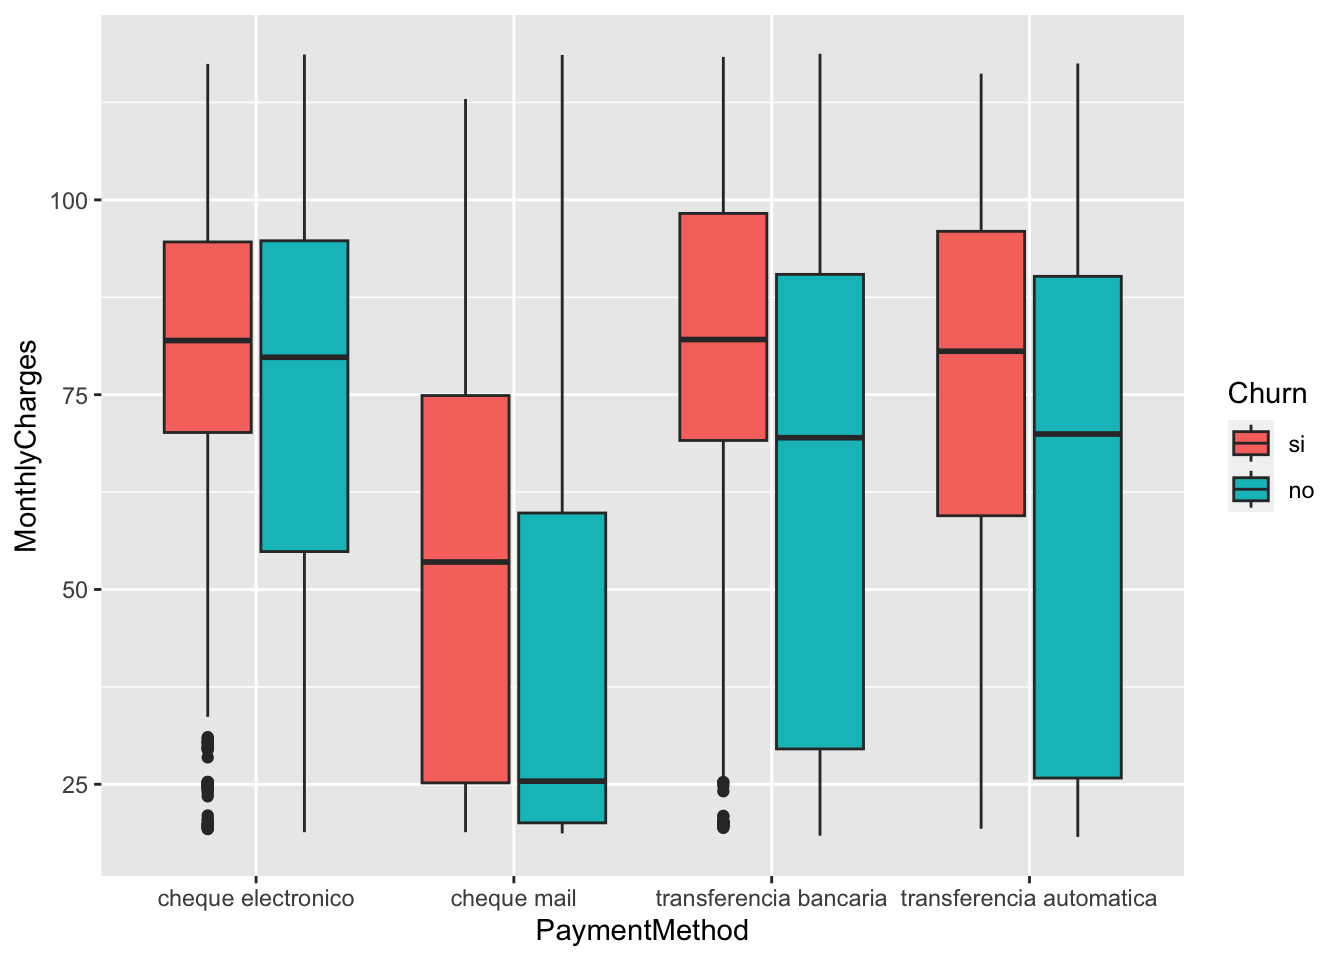
\includegraphics{model_Room_8_files/figure-latex/unnamed-chunk-28-1.pdf}

En promedio el gasto total en el servicio de telecomunicaciones para los
individuos que salieron del plan es inferior por usuario en alrededor de
USD 1000. Para los usuarios que salieron del servicio se evidencia datos
atípicos elevados que alcanzan los valores máximos de los usarios que no
salieron del servicio. Cabe señalar que, para los usuarios que no
abandoron el servicio su extipendio total del plan se concentra entre el
rango intercuartílico. Adicionalmente, se observa que la variable gasto
total cuenta con 11 valores perdidos.

\hypertarget{eda-multivariado-entre-monthlycharges-vs-dependents-vs-churn}{%
\paragraph{Eda Multivariado entre MonthlyCharges vs Dependents vs
Churn}\label{eda-multivariado-entre-monthlycharges-vs-dependents-vs-churn}}

\begin{Shaded}
\begin{Highlighting}[]
\NormalTok{data }\SpecialCharTok{\%\textgreater{}\%}  \FunctionTok{group\_by}\NormalTok{(Churn,Dependents) }\SpecialCharTok{\%\textgreater{}\%} 
    \FunctionTok{summarise}\NormalTok{(}\AttributeTok{n =} \FunctionTok{n}\NormalTok{(),}
            \AttributeTok{promedio =} \FunctionTok{mean}\NormalTok{(MonthlyCharges,}\AttributeTok{na.rm =}\NormalTok{ T),}
            \AttributeTok{n\_missing =} \FunctionTok{sum}\NormalTok{(}\FunctionTok{is.na}\NormalTok{(MonthlyCharges)),}
            \AttributeTok{desv =} \FunctionTok{sd}\NormalTok{(MonthlyCharges, }\AttributeTok{na.rm =}\NormalTok{T)) }\OtherTok{{-}\textgreater{}}\NormalTok{ t5}
\end{Highlighting}
\end{Shaded}

\begin{verbatim}
## `summarise()` has grouped output by 'Churn'. You can override using the
## `.groups` argument.
\end{verbatim}

\begin{Shaded}
\begin{Highlighting}[]
\NormalTok{t5}
\end{Highlighting}
\end{Shaded}

\begin{verbatim}
## # A tibble: 4 x 6
## # Groups:   Churn [2]
##   Churn Dependents     n promedio n_missing  desv
##   <fct> <fct>      <int>    <dbl>     <int> <dbl>
## 1 si    si           326     72.9         0  25.8
## 2 si    No          1543     74.8         0  24.4
## 3 no    si          1784     57.1         0  31.6
## 4 no    No          3390     63.5         0  30.6
\end{verbatim}

\begin{Shaded}
\begin{Highlighting}[]
\NormalTok{data }\SpecialCharTok{\%\textgreater{}\%}
  \FunctionTok{ggplot}\NormalTok{(}\FunctionTok{aes}\NormalTok{(}\AttributeTok{x =}\NormalTok{ Churn, }\AttributeTok{y =}\NormalTok{ MonthlyCharges, }\AttributeTok{fill =}\NormalTok{ Dependents)) }\SpecialCharTok{+}
  \FunctionTok{geom\_boxplot}\NormalTok{() }\SpecialCharTok{+}
  \FunctionTok{stat\_summary}\NormalTok{(}\AttributeTok{fun =}\NormalTok{ mean, }\AttributeTok{geom =} \StringTok{"point"}\NormalTok{, }\AttributeTok{shape =} \DecValTok{3}\NormalTok{, }\AttributeTok{size =} \DecValTok{3}\NormalTok{, }\AttributeTok{color =} \StringTok{"white"}\NormalTok{, }\AttributeTok{position =} \FunctionTok{position\_dodge}\NormalTok{(}\AttributeTok{width =} \FloatTok{0.75}\NormalTok{)) }\SpecialCharTok{+}
  \FunctionTok{labs}\NormalTok{(}\AttributeTok{title =} \StringTok{"Monthtly Charges for Dependents vs Churn"}\NormalTok{,}
       \AttributeTok{x =} \StringTok{"Churn"}\NormalTok{,}
       \AttributeTok{y =} \StringTok{"Monthly Charges"}\NormalTok{)}
\end{Highlighting}
\end{Shaded}

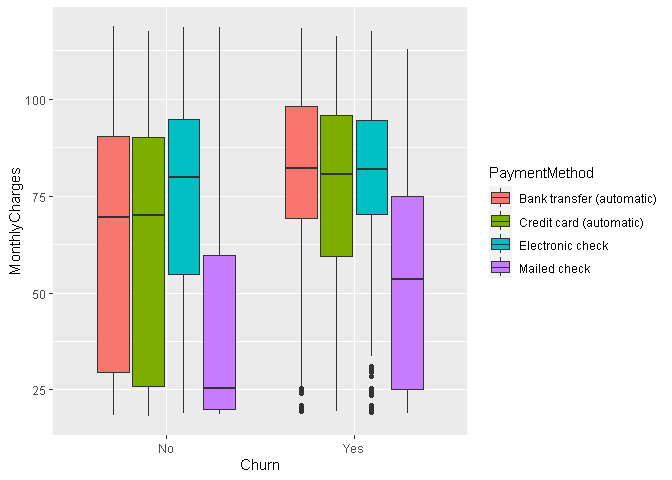
\includegraphics{model_Room_8_files/figure-latex/unnamed-chunk-29-1.pdf}

La distribución del gasto mensual de aquellos individuos que no salieron
del plan se concentra dentro del cuartil 1 y cuartil 3, además entre el
máximo y mínimo de los que dejaron el servicio respecto de los que se
quedaron no se verifica mayor diferencia. Es importante destacar que,
tanto el promedio como la mediana del pago mensual es superior en los
individuos que salieron del plan de los que se quedaron, no obstante no
se verifica mayor diferencia respecto de contar o no con dependientes en
los usuarios que abandonaron el plan.

\hypertarget{room-9}{%
\subsubsection{Room 9}\label{room-9}}

\hypertarget{room-10}{%
\subsubsection{Room 10}\label{room-10}}

\hypertarget{matriz-de-correlaciuxf3n}{%
\subsubsection{Matriz de Correlación}\label{matriz-de-correlaciuxf3n}}

\begin{Shaded}
\begin{Highlighting}[]
\CommentTok{\#data \%\textgreater{}\%  select({-}customerID) \%\textgreater{}\% GGally::ggpairs()}
\NormalTok{data }\SpecialCharTok{\%\textgreater{}\%}  \FunctionTok{select\_if}\NormalTok{(}\FunctionTok{where}\NormalTok{(is.numeric)) }\SpecialCharTok{\%\textgreater{}\%}\NormalTok{ GGally}\SpecialCharTok{::}\FunctionTok{ggpairs}\NormalTok{()}
\end{Highlighting}
\end{Shaded}

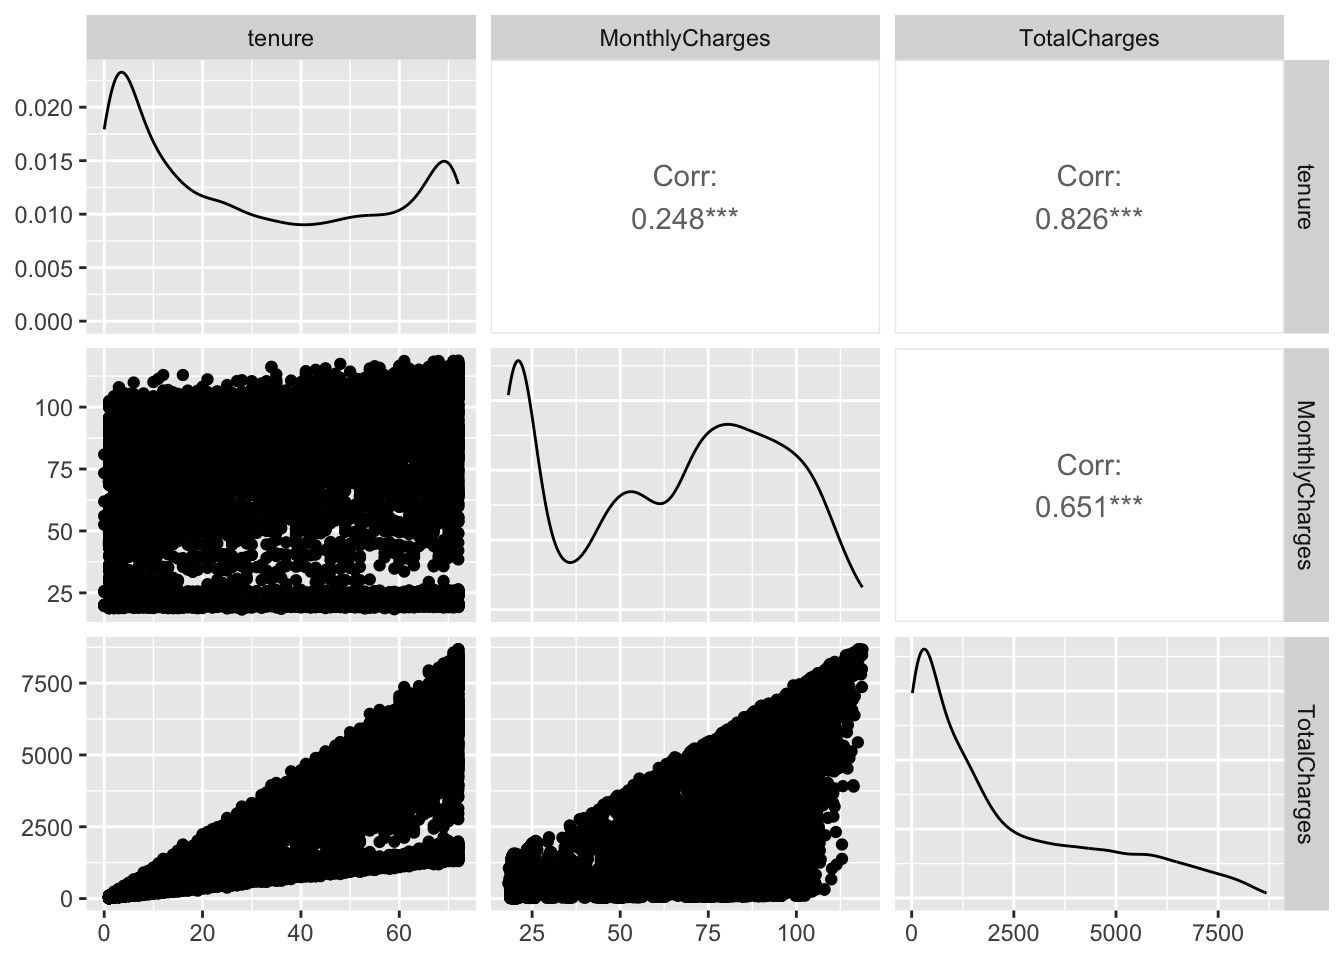
\includegraphics{model_Room_8_files/figure-latex/unnamed-chunk-30-1.pdf}

Según el gráfico anterior existe una alta correlación positiva entre las
variables TotalChanges y tenure, con 0.826, seguida de la correlación
entre las variables TotalChages y MonthyChanges, con una correlación
moderada de 0.651.

\textbf{MODELAMIENTO}

\hypertarget{train---test-split}{%
\subsubsection{Train - Test Split}\label{train---test-split}}

\begin{Shaded}
\begin{Highlighting}[]
\CommentTok{\#data \%\textgreater{}\% select({-}customerID) {-}\textgreater{} data}

\FunctionTok{set.seed}\NormalTok{(}\DecValTok{1234}\NormalTok{) }\CommentTok{\# Semilla para aleatorios}
\NormalTok{split }\OtherTok{\textless{}{-}}\NormalTok{ data }\SpecialCharTok{\%\textgreater{}\%}
\FunctionTok{initial\_split}\NormalTok{(}
\AttributeTok{prop =} \FloatTok{0.8}\NormalTok{, }\CommentTok{\# Porcentaje al train}
\AttributeTok{strata =}\NormalTok{ Churn }\CommentTok{\# Estratificación del muestreo}
\NormalTok{)}
\end{Highlighting}
\end{Shaded}

\hypertarget{data-de-entrenamiento}{%
\subsubsection{Data de entrenamiento}\label{data-de-entrenamiento}}

\begin{Shaded}
\begin{Highlighting}[]
\NormalTok{train }\OtherTok{\textless{}{-}} \FunctionTok{training}\NormalTok{(split)}
\FunctionTok{dim}\NormalTok{(train)}
\end{Highlighting}
\end{Shaded}

\begin{verbatim}
## [1] 5634   21
\end{verbatim}

\hypertarget{data-de-prueba-test}{%
\subsubsection{Data de prueba (test)}\label{data-de-prueba-test}}

\begin{Shaded}
\begin{Highlighting}[]
\NormalTok{test }\OtherTok{\textless{}{-}} \FunctionTok{testing}\NormalTok{(split)}
\FunctionTok{dim}\NormalTok{(test)}
\end{Highlighting}
\end{Shaded}

\begin{verbatim}
## [1] 1409   21
\end{verbatim}

\hypertarget{preprocesamiento}{%
\subsubsection{Preprocesamiento}\label{preprocesamiento}}

\hypertarget{receipe-y-balanceo-de-datos}{%
\paragraph{Receipe y Balanceo de
datos}\label{receipe-y-balanceo-de-datos}}

\begin{Shaded}
\begin{Highlighting}[]
\NormalTok{receta }\OtherTok{\textless{}{-}}\NormalTok{ train }\SpecialCharTok{\%\textgreater{}\%}
\FunctionTok{recipe}\NormalTok{(Churn }\SpecialCharTok{\textasciitilde{}}\NormalTok{ . ) }\SpecialCharTok{\%\textgreater{}\%} \DocumentationTok{\#\# Crea la receta}
\DocumentationTok{\#\# Eliminar variables que no usaremos}
\FunctionTok{step\_rm}\NormalTok{(customerID) }\SpecialCharTok{\%\textgreater{}\%}
\DocumentationTok{\#\# Crear nuevas variables (insight desde el EDA)}
\CommentTok{\# step\_mutate( account\_length\_anio= account\_length/12 )}
\DocumentationTok{\#\# Imputar los datos}
\CommentTok{\# step\_impute\_mean()}
\FunctionTok{step\_impute\_knn}\NormalTok{(TotalCharges ) }\SpecialCharTok{\%\textgreater{}\%}
\DocumentationTok{\#\# Estandarizacion/Normalizacion de numericas}
\FunctionTok{step\_normalize}\NormalTok{( }\FunctionTok{all\_numeric}\NormalTok{(), }\SpecialCharTok{{-}}\FunctionTok{all\_outcomes}\NormalTok{()) }\SpecialCharTok{\%\textgreater{}\%}
\DocumentationTok{\#\# Crear una categoría "otros" que agrupe a categorias pequeñas}
\FunctionTok{step\_other}\NormalTok{(}\FunctionTok{all\_nominal}\NormalTok{(), }\SpecialCharTok{{-}}\FunctionTok{all\_outcomes}\NormalTok{() , }\AttributeTok{threshold =} \FloatTok{0.07}\NormalTok{, }\AttributeTok{other =} \StringTok{"otros"}\NormalTok{) }\SpecialCharTok{\%\textgreater{}\%}
\DocumentationTok{\#\# Crear una categoría "new" para observaciones con labels "no muestreados"}
\FunctionTok{step\_novel}\NormalTok{(}\FunctionTok{all\_nominal}\NormalTok{(), }\SpecialCharTok{{-}}\FunctionTok{all\_outcomes}\NormalTok{() , }\AttributeTok{new\_level =} \StringTok{"new"}\NormalTok{) }\SpecialCharTok{\%\textgreater{}\%}
\DocumentationTok{\#\# Crear variables indicadoras para cada categoría}
\FunctionTok{step\_dummy}\NormalTok{(}\FunctionTok{all\_nominal}\NormalTok{(), }\SpecialCharTok{{-}}\FunctionTok{all\_outcomes}\NormalTok{() ) }\SpecialCharTok{\%\textgreater{}\%} \CommentTok{\# Dummy}
\DocumentationTok{\#\# Eliminar automáticamente variables con alta correlacion}
\DocumentationTok{\#\# para evitar la multicolinealidad xi \textasciitilde{} xj}
\CommentTok{\# step\_corr(all\_numeric(), {-}all\_outcomes(), threshold = 0.9) \%\textgreater{}\%}
\DocumentationTok{\#\# Tambien podemos eliminar variables con multicolinealidad "a mano"}
\CommentTok{\#step\_rm(total\_day\_charge, total\_eve\_charge,}
\CommentTok{\#total\_night\_charge, total\_intl\_charge) \%\textgreater{}\% \# Eliminar}
\DocumentationTok{\#\# Eliminar columnas con varianza cercana a cero}
\FunctionTok{step\_nzv}\NormalTok{(}\FunctionTok{all\_predictors}\NormalTok{()) }\SpecialCharTok{\%\textgreater{}\%} 
\NormalTok{themis}\SpecialCharTok{::}\FunctionTok{step\_upsample}\NormalTok{(Churn, }\AttributeTok{over\_ratio =} \FloatTok{0.9}\NormalTok{, }\AttributeTok{skip=} \ConstantTok{TRUE}\NormalTok{, }\AttributeTok{seed=} \DecValTok{123}\NormalTok{)  }
\end{Highlighting}
\end{Shaded}

\hypertarget{entrenamiento-y-ajuste-de-hiperparuxe1metro}{%
\paragraph{Entrenamiento y ajuste de
Hiperparámetro}\label{entrenamiento-y-ajuste-de-hiperparuxe1metro}}

\begin{Shaded}
\begin{Highlighting}[]
\FunctionTok{set.seed}\NormalTok{(}\DecValTok{1234}\NormalTok{)}
\NormalTok{cv }\OtherTok{\textless{}{-}} \FunctionTok{vfold\_cv}\NormalTok{(train, }\AttributeTok{v =} \DecValTok{5}\NormalTok{, }\AttributeTok{repeats =} \DecValTok{1}\NormalTok{, }\AttributeTok{strata =}\NormalTok{ Churn)}
\NormalTok{cv}
\end{Highlighting}
\end{Shaded}

\begin{verbatim}
## #  5-fold cross-validation using stratification 
## # A tibble: 5 x 2
##   splits              id   
##   <list>              <chr>
## 1 <split [4507/1127]> Fold1
## 2 <split [4507/1127]> Fold2
## 3 <split [4507/1127]> Fold3
## 4 <split [4507/1127]> Fold4
## 5 <split [4508/1126]> Fold5
\end{verbatim}

\hypertarget{muxe9tricas}{%
\subsubsection{Métricas}\label{muxe9tricas}}

\begin{Shaded}
\begin{Highlighting}[]
\NormalTok{metricas }\OtherTok{\textless{}{-}} \FunctionTok{metric\_set}\NormalTok{(accuracy, sens, spec, bal\_accuracy)}
\NormalTok{metricas}
\end{Highlighting}
\end{Shaded}

\begin{verbatim}
## A metric set, consisting of:
## - `accuracy()`, a class metric     | direction: maximize
## - `sens()`, a class metric         | direction: maximize
## - `spec()`, a class metric         | direction: maximize
## - `bal_accuracy()`, a class metric | direction: maximize
\end{verbatim}

\textbf{Modelamiento - Random Forest}

\emph{Especificacion del modelo}

\begin{Shaded}
\begin{Highlighting}[]
\NormalTok{rf\_sp }\OtherTok{\textless{}{-}}
  \FunctionTok{rand\_forest}\NormalTok{(}
  \AttributeTok{mtry =} \FunctionTok{tune}\NormalTok{(), }\AttributeTok{trees =} \FunctionTok{tune}\NormalTok{(), }\AttributeTok{min\_n =} \FunctionTok{tune}\NormalTok{() ) }\SpecialCharTok{\%\textgreater{}\%}
  \FunctionTok{set\_engine}\NormalTok{(}\StringTok{"ranger"}\NormalTok{, }\AttributeTok{importance =} \StringTok{"impurity"}\NormalTok{) }\SpecialCharTok{\%\textgreater{}\%}
  \FunctionTok{set\_mode}\NormalTok{(}\StringTok{"classification"}\NormalTok{)}
\end{Highlighting}
\end{Shaded}

\emph{Work Flow}

\begin{Shaded}
\begin{Highlighting}[]
\NormalTok{rf\_wflow }\OtherTok{\textless{}{-}}
  \FunctionTok{workflow}\NormalTok{() }\SpecialCharTok{\%\textgreater{}\%}
  \FunctionTok{add\_recipe}\NormalTok{(receta) }\SpecialCharTok{\%\textgreater{}\%}
  \FunctionTok{add\_model}\NormalTok{(rf\_sp) }
\NormalTok{  rf\_wflow}
\end{Highlighting}
\end{Shaded}

\begin{verbatim}
## == Workflow ====================================================================
## Preprocessor: Recipe
## Model: rand_forest()
## 
## -- Preprocessor ----------------------------------------------------------------
## 8 Recipe Steps
## 
## * step_rm()
## * step_impute_knn()
## * step_normalize()
## * step_other()
## * step_novel()
## * step_dummy()
## * step_nzv()
## * step_upsample()
## 
## -- Model -----------------------------------------------------------------------
## Random Forest Model Specification (classification)
## 
## Main Arguments:
##   mtry = tune()
##   trees = tune()
##   min_n = tune()
## 
## Engine-Specific Arguments:
##   importance = impurity
## 
## Computational engine: ranger
\end{verbatim}

\emph{Afinamiento de Hiperpárametros}

\begin{Shaded}
\begin{Highlighting}[]
\FunctionTok{set.seed}\NormalTok{(}\DecValTok{123}\NormalTok{)}
\NormalTok{rf\_grid }\OtherTok{\textless{}{-}}\NormalTok{ rf\_sp }\SpecialCharTok{\%\textgreater{}\%}
\DocumentationTok{\#\# preguntamos los parametros tuneables del modelo}
\FunctionTok{parameters}\NormalTok{() }\SpecialCharTok{\%\textgreater{}\%}
\DocumentationTok{\#\# Vamos a definir un rango para el min\_n y mtry}
\FunctionTok{update}\NormalTok{(}\AttributeTok{min\_n=} \FunctionTok{min\_n}\NormalTok{( }\AttributeTok{range=} \FunctionTok{c}\NormalTok{(}\DecValTok{70}\NormalTok{, }\DecValTok{170}\NormalTok{)),}
\AttributeTok{mtry=} \FunctionTok{mtry}\NormalTok{( }\AttributeTok{range=} \FunctionTok{c}\NormalTok{(}\DecValTok{4}\NormalTok{, }\DecValTok{7}\NormalTok{))) }\SpecialCharTok{\%\textgreater{}\%}
\FunctionTok{grid\_latin\_hypercube}\NormalTok{(}\AttributeTok{size =} \DecValTok{10}\NormalTok{) }\CommentTok{\#preguntar como se construye la malla}
\end{Highlighting}
\end{Shaded}

\begin{verbatim}
## Warning: `parameters.model_spec()` was deprecated in tune 0.1.6.9003.
## i Please use `hardhat::extract_parameter_set_dials()` instead.
## This warning is displayed once every 8 hours.
## Call `lifecycle::last_lifecycle_warnings()` to see where this warning was
## generated.
\end{verbatim}

\#\#\#Paralelización

\begin{Shaded}
\begin{Highlighting}[]
\CommentTok{\#parallel::detectCores(logical=FALSE)}
\end{Highlighting}
\end{Shaded}

\emph{Entrenamiento de Malla de Búsqueda en la Crossvalidation}

\begin{Shaded}
\begin{Highlighting}[]
\FunctionTok{set.seed}\NormalTok{(}\DecValTok{123}\NormalTok{)}
\NormalTok{rf\_tuned }\OtherTok{\textless{}{-}} \FunctionTok{tune\_grid}\NormalTok{(}
\NormalTok{        rf\_wflow, }\DocumentationTok{\#\# Modelo}
        \AttributeTok{resamples=}\NormalTok{ cv, }\DocumentationTok{\#\# Crossvalidation}
        \AttributeTok{grid =}\NormalTok{ rf\_grid, }\DocumentationTok{\#\# Malla de Busqueda}
        \AttributeTok{metrics =}\NormalTok{ metricas, }\DocumentationTok{\#\# Metricas}
        \AttributeTok{control=} \FunctionTok{control\_grid}\NormalTok{(}\AttributeTok{allow\_par =}\NormalTok{ T, }\AttributeTok{save\_pred =}\NormalTok{ T) }\DocumentationTok{\#\# Paralel y Pred}
\NormalTok{)}
\end{Highlighting}
\end{Shaded}

\begin{verbatim}
## Warning: package 'themis' was built under R version 4.3.3
\end{verbatim}

\begin{Shaded}
\begin{Highlighting}[]
\NormalTok{rf\_tuned}
\end{Highlighting}
\end{Shaded}

\begin{verbatim}
## # Tuning results
## # 5-fold cross-validation using stratification 
## # A tibble: 5 x 5
##   splits              id    .metrics          .notes           .predictions
##   <list>              <chr> <list>            <list>           <list>      
## 1 <split [4507/1127]> Fold1 <tibble [40 x 7]> <tibble [0 x 3]> <tibble>    
## 2 <split [4507/1127]> Fold2 <tibble [40 x 7]> <tibble [0 x 3]> <tibble>    
## 3 <split [4507/1127]> Fold3 <tibble [40 x 7]> <tibble [0 x 3]> <tibble>    
## 4 <split [4507/1127]> Fold4 <tibble [40 x 7]> <tibble [0 x 3]> <tibble>    
## 5 <split [4508/1126]> Fold5 <tibble [40 x 7]> <tibble [0 x 3]> <tibble>
\end{verbatim}

\emph{Evaluación de modelos Evaluamos que modelo resulto mejor}

\begin{Shaded}
\begin{Highlighting}[]
\FunctionTok{show\_best}\NormalTok{(rf\_tuned, }\AttributeTok{metric =} \StringTok{\textquotesingle{}accuracy\textquotesingle{}}\NormalTok{, }\AttributeTok{n =} \DecValTok{10}\NormalTok{)}
\end{Highlighting}
\end{Shaded}

\begin{verbatim}
## # A tibble: 10 x 9
##     mtry trees min_n .metric  .estimator  mean     n std_err .config            
##    <int> <int> <int> <chr>    <chr>      <dbl> <int>   <dbl> <chr>              
##  1     5   325    83 accuracy binary     0.768     5 0.00959 Preprocessor1_Mode~
##  2     4  1370   116 accuracy binary     0.768     5 0.00891 Preprocessor1_Mode~
##  3     6   950   130 accuracy binary     0.768     5 0.0104  Preprocessor1_Mode~
##  4     7   773    80 accuracy binary     0.768     5 0.00870 Preprocessor1_Mode~
##  5     6   467    91 accuracy binary     0.767     5 0.00889 Preprocessor1_Mode~
##  6     5  1904   126 accuracy binary     0.767     5 0.0100  Preprocessor1_Mode~
##  7     5  1441   106 accuracy binary     0.766     5 0.0103  Preprocessor1_Mode~
##  8     6  1124   162 accuracy binary     0.766     5 0.00995 Preprocessor1_Mode~
##  9     6  1737   158 accuracy binary     0.766     5 0.00977 Preprocessor1_Mode~
## 10     5    70   144 accuracy binary     0.764     5 0.00938 Preprocessor1_Mode~
\end{verbatim}

\begin{Shaded}
\begin{Highlighting}[]
\FunctionTok{show\_best}\NormalTok{(rf\_tuned, }\AttributeTok{metric =} \StringTok{\textquotesingle{}sens\textquotesingle{}}\NormalTok{, }\AttributeTok{n =} \DecValTok{10}\NormalTok{)}
\end{Highlighting}
\end{Shaded}

\begin{verbatim}
## # A tibble: 10 x 9
##     mtry trees min_n .metric .estimator  mean     n std_err .config             
##    <int> <int> <int> <chr>   <chr>      <dbl> <int>   <dbl> <chr>               
##  1     4  1370   116 sens    binary     0.741     5 0.0157  Preprocessor1_Model~
##  2     6  1737   158 sens    binary     0.738     5 0.0115  Preprocessor1_Model~
##  3     6  1124   162 sens    binary     0.738     5 0.0124  Preprocessor1_Model~
##  4     5    70   144 sens    binary     0.737     5 0.0132  Preprocessor1_Model~
##  5     5  1904   126 sens    binary     0.737     5 0.0132  Preprocessor1_Model~
##  6     6   950   130 sens    binary     0.734     5 0.0128  Preprocessor1_Model~
##  7     5  1441   106 sens    binary     0.732     5 0.0137  Preprocessor1_Model~
##  8     5   325    83 sens    binary     0.728     5 0.0133  Preprocessor1_Model~
##  9     6   467    91 sens    binary     0.726     5 0.00936 Preprocessor1_Model~
## 10     7   773    80 sens    binary     0.722     5 0.00983 Preprocessor1_Model~
\end{verbatim}

\begin{Shaded}
\begin{Highlighting}[]
\FunctionTok{show\_best}\NormalTok{(rf\_tuned, }\AttributeTok{metric =} \StringTok{\textquotesingle{}spec\textquotesingle{}}\NormalTok{, }\AttributeTok{n =} \DecValTok{10}\NormalTok{)}
\end{Highlighting}
\end{Shaded}

\begin{verbatim}
## # A tibble: 10 x 9
##     mtry trees min_n .metric .estimator  mean     n std_err .config             
##    <int> <int> <int> <chr>   <chr>      <dbl> <int>   <dbl> <chr>               
##  1     7   773    80 spec    binary     0.784     5 0.00840 Preprocessor1_Model~
##  2     5   325    83 spec    binary     0.783     5 0.00840 Preprocessor1_Model~
##  3     6   467    91 spec    binary     0.781     5 0.00887 Preprocessor1_Model~
##  4     6   950   130 spec    binary     0.780     5 0.0102  Preprocessor1_Model~
##  5     5  1441   106 spec    binary     0.778     5 0.00922 Preprocessor1_Model~
##  6     4  1370   116 spec    binary     0.778     5 0.00723 Preprocessor1_Model~
##  7     5  1904   126 spec    binary     0.777     5 0.00930 Preprocessor1_Model~
##  8     6  1124   162 spec    binary     0.777     5 0.00959 Preprocessor1_Model~
##  9     6  1737   158 spec    binary     0.777     5 0.00938 Preprocessor1_Model~
## 10     5    70   144 spec    binary     0.774     5 0.00843 Preprocessor1_Model~
\end{verbatim}

\begin{Shaded}
\begin{Highlighting}[]
\FunctionTok{show\_best}\NormalTok{(rf\_tuned, }\AttributeTok{metric =} \StringTok{\textquotesingle{}bal\_accuracy\textquotesingle{}}\NormalTok{, }\AttributeTok{n =} \DecValTok{10}\NormalTok{)}
\end{Highlighting}
\end{Shaded}

\begin{verbatim}
## # A tibble: 10 x 9
##     mtry trees min_n .metric      .estimator  mean     n std_err .config        
##    <int> <int> <int> <chr>        <chr>      <dbl> <int>   <dbl> <chr>          
##  1     4  1370   116 bal_accuracy binary     0.760     5 0.0109  Preprocessor1_~
##  2     5  1904   126 bal_accuracy binary     0.757     5 0.0109  Preprocessor1_~
##  3     6  1124   162 bal_accuracy binary     0.757     5 0.0105  Preprocessor1_~
##  4     6  1737   158 bal_accuracy binary     0.757     5 0.0102  Preprocessor1_~
##  5     6   950   130 bal_accuracy binary     0.757     5 0.0110  Preprocessor1_~
##  6     5   325    83 bal_accuracy binary     0.755     5 0.0107  Preprocessor1_~
##  7     5    70   144 bal_accuracy binary     0.755     5 0.0105  Preprocessor1_~
##  8     5  1441   106 bal_accuracy binary     0.755     5 0.0113  Preprocessor1_~
##  9     6   467    91 bal_accuracy binary     0.754     5 0.00898 Preprocessor1_~
## 10     7   773    80 bal_accuracy binary     0.753     5 0.00902 Preprocessor1_~
\end{verbatim}

Revisando los resultados de las métricas de evaluación del modelo y
considerando que es de interés para le empresa contar con la mejor
estimación de los individuos que realmente abandonan el servicio se
selecciona como referencia los hiperpárametros del modelo número 6 que
presenta los mejores resultados en sensibilidad, para ajustar el modelo
final.

\emph{Nueva Malla de Búsqueda}

\begin{Shaded}
\begin{Highlighting}[]
\FunctionTok{set.seed}\NormalTok{(}\DecValTok{123}\NormalTok{)}

\NormalTok{rf\_grid\_2 }\OtherTok{\textless{}{-}} \FunctionTok{crossing}\NormalTok{(}
  \AttributeTok{min\_n =} \FunctionTok{seq}\NormalTok{(}\DecValTok{114}\NormalTok{, }\DecValTok{118}\NormalTok{, }\DecValTok{2}\NormalTok{),}
  \AttributeTok{mtry =} \FunctionTok{c}\NormalTok{(}\DecValTok{4}\NormalTok{, }\DecValTok{5}\NormalTok{),}
  \AttributeTok{trees=} \FunctionTok{seq}\NormalTok{(}\DecValTok{1270}\NormalTok{, }\DecValTok{1570}\NormalTok{, }\DecValTok{100}\NormalTok{)}
\NormalTok{)}

\NormalTok{rf\_grid\_2}
\end{Highlighting}
\end{Shaded}

\begin{verbatim}
## # A tibble: 24 x 3
##    min_n  mtry trees
##    <dbl> <dbl> <dbl>
##  1   114     4  1270
##  2   114     4  1370
##  3   114     4  1470
##  4   114     4  1570
##  5   114     5  1270
##  6   114     5  1370
##  7   114     5  1470
##  8   114     5  1570
##  9   116     4  1270
## 10   116     4  1370
## # i 14 more rows
\end{verbatim}

\emph{Entrenamiento de Malla de Busqueda en la Crossvalidation}

\begin{Shaded}
\begin{Highlighting}[]
\FunctionTok{set.seed}\NormalTok{(}\DecValTok{123}\NormalTok{)}
\NormalTok{rf\_tuned\_2 }\OtherTok{\textless{}{-}} \FunctionTok{tune\_grid}\NormalTok{(}
\NormalTok{  rf\_wflow, }\DocumentationTok{\#\# Modelo}
  \AttributeTok{resamples=}\NormalTok{ cv, }\DocumentationTok{\#\# Crossvalidation}
  \AttributeTok{grid =}\NormalTok{ rf\_grid\_2, }\DocumentationTok{\#\# Malla de Busqueda}
  \AttributeTok{metrics =}\NormalTok{ metricas, }\DocumentationTok{\#\# Metricas}
  \AttributeTok{control=} \FunctionTok{control\_grid}\NormalTok{(}\AttributeTok{allow\_par =}\NormalTok{ T, }\AttributeTok{save\_pred =}\NormalTok{ T) }\DocumentationTok{\#\# Paralel y Pred}
\NormalTok{)}
\NormalTok{rf\_tuned\_2}
\end{Highlighting}
\end{Shaded}

\begin{verbatim}
## # Tuning results
## # 5-fold cross-validation using stratification 
## # A tibble: 5 x 5
##   splits              id    .metrics          .notes           .predictions
##   <list>              <chr> <list>            <list>           <list>      
## 1 <split [4507/1127]> Fold1 <tibble [96 x 7]> <tibble [0 x 3]> <tibble>    
## 2 <split [4507/1127]> Fold2 <tibble [96 x 7]> <tibble [0 x 3]> <tibble>    
## 3 <split [4507/1127]> Fold3 <tibble [96 x 7]> <tibble [0 x 3]> <tibble>    
## 4 <split [4507/1127]> Fold4 <tibble [96 x 7]> <tibble [0 x 3]> <tibble>    
## 5 <split [4508/1126]> Fold5 <tibble [96 x 7]> <tibble [0 x 3]> <tibble>
\end{verbatim}

Evaluamos que modelo resulto mejor de la segunda grilla de
hiperpárametros

\begin{Shaded}
\begin{Highlighting}[]
\FunctionTok{show\_best}\NormalTok{(rf\_tuned\_2, }\AttributeTok{metric =} \StringTok{\textquotesingle{}accuracy\textquotesingle{}}\NormalTok{, }\AttributeTok{n =} \DecValTok{10}\NormalTok{)}
\end{Highlighting}
\end{Shaded}

\begin{verbatim}
## # A tibble: 10 x 9
##     mtry trees min_n .metric  .estimator  mean     n std_err .config            
##    <dbl> <dbl> <dbl> <chr>    <chr>      <dbl> <int>   <dbl> <chr>              
##  1     4  1470   116 accuracy binary     0.768     5 0.00952 Preprocessor1_Mode~
##  2     4  1270   118 accuracy binary     0.768     5 0.00880 Preprocessor1_Mode~
##  3     5  1270   114 accuracy binary     0.767     5 0.00949 Preprocessor1_Mode~
##  4     4  1270   116 accuracy binary     0.767     5 0.00920 Preprocessor1_Mode~
##  5     4  1570   118 accuracy binary     0.767     5 0.00875 Preprocessor1_Mode~
##  6     4  1470   118 accuracy binary     0.767     5 0.0101  Preprocessor1_Mode~
##  7     4  1570   116 accuracy binary     0.767     5 0.00937 Preprocessor1_Mode~
##  8     5  1470   114 accuracy binary     0.767     5 0.00953 Preprocessor1_Mode~
##  9     4  1370   118 accuracy binary     0.767     5 0.00987 Preprocessor1_Mode~
## 10     5  1370   118 accuracy binary     0.767     5 0.0100  Preprocessor1_Mode~
\end{verbatim}

\begin{Shaded}
\begin{Highlighting}[]
\FunctionTok{show\_best}\NormalTok{(rf\_tuned\_2, }\AttributeTok{metric =} \StringTok{\textquotesingle{}sens\textquotesingle{}}\NormalTok{, }\AttributeTok{n =} \DecValTok{10}\NormalTok{)}
\end{Highlighting}
\end{Shaded}

\begin{verbatim}
## # A tibble: 10 x 9
##     mtry trees min_n .metric .estimator  mean     n std_err .config             
##    <dbl> <dbl> <dbl> <chr>   <chr>      <dbl> <int>   <dbl> <chr>               
##  1     4  1570   116 sens    binary     0.738     5  0.0140 Preprocessor1_Model~
##  2     4  1470   118 sens    binary     0.738     5  0.0163 Preprocessor1_Model~
##  3     4  1270   116 sens    binary     0.737     5  0.0152 Preprocessor1_Model~
##  4     4  1370   116 sens    binary     0.737     5  0.0159 Preprocessor1_Model~
##  5     4  1270   118 sens    binary     0.737     5  0.0139 Preprocessor1_Model~
##  6     4  1370   114 sens    binary     0.736     5  0.0137 Preprocessor1_Model~
##  7     4  1570   114 sens    binary     0.736     5  0.0145 Preprocessor1_Model~
##  8     5  1470   114 sens    binary     0.736     5  0.0125 Preprocessor1_Model~
##  9     4  1470   116 sens    binary     0.736     5  0.0159 Preprocessor1_Model~
## 10     4  1470   114 sens    binary     0.735     5  0.0140 Preprocessor1_Model~
\end{verbatim}

\begin{Shaded}
\begin{Highlighting}[]
\FunctionTok{show\_best}\NormalTok{(rf\_tuned\_2, }\AttributeTok{metric =} \StringTok{\textquotesingle{}spec\textquotesingle{}}\NormalTok{, }\AttributeTok{n =} \DecValTok{10}\NormalTok{)}
\end{Highlighting}
\end{Shaded}

\begin{verbatim}
## # A tibble: 10 x 9
##     mtry trees min_n .metric .estimator  mean     n std_err .config             
##    <dbl> <dbl> <dbl> <chr>   <chr>      <dbl> <int>   <dbl> <chr>               
##  1     4  1470   116 spec    binary     0.780     5 0.00763 Preprocessor1_Model~
##  2     5  1370   118 spec    binary     0.780     5 0.00931 Preprocessor1_Model~
##  3     4  1370   118 spec    binary     0.779     5 0.00851 Preprocessor1_Model~
##  4     4  1570   118 spec    binary     0.779     5 0.00764 Preprocessor1_Model~
##  5     5  1270   114 spec    binary     0.779     5 0.00883 Preprocessor1_Model~
##  6     5  1570   118 spec    binary     0.779     5 0.00860 Preprocessor1_Model~
##  7     5  1470   116 spec    binary     0.779     5 0.00917 Preprocessor1_Model~
##  8     4  1270   118 spec    binary     0.779     5 0.00738 Preprocessor1_Model~
##  9     5  1470   114 spec    binary     0.778     5 0.00899 Preprocessor1_Model~
## 10     4  1570   114 spec    binary     0.778     5 0.00868 Preprocessor1_Model~
\end{verbatim}

\begin{Shaded}
\begin{Highlighting}[]
\FunctionTok{show\_best}\NormalTok{(rf\_tuned\_2, }\AttributeTok{metric =} \StringTok{\textquotesingle{}bal\_accuracy\textquotesingle{}}\NormalTok{, }\AttributeTok{n =} \DecValTok{10}\NormalTok{)}
\end{Highlighting}
\end{Shaded}

\begin{verbatim}
## # A tibble: 10 x 9
##     mtry trees min_n .metric      .estimator  mean     n std_err .config        
##    <dbl> <dbl> <dbl> <chr>        <chr>      <dbl> <int>   <dbl> <chr>          
##  1     4  1570   116 bal_accuracy binary     0.758     5  0.0107 Preprocessor1_~
##  2     4  1470   116 bal_accuracy binary     0.758     5  0.0114 Preprocessor1_~
##  3     4  1270   118 bal_accuracy binary     0.758     5  0.0103 Preprocessor1_~
##  4     4  1470   118 bal_accuracy binary     0.758     5  0.0119 Preprocessor1_~
##  5     4  1270   116 bal_accuracy binary     0.758     5  0.0110 Preprocessor1_~
##  6     4  1370   116 bal_accuracy binary     0.757     5  0.0113 Preprocessor1_~
##  7     5  1270   114 bal_accuracy binary     0.757     5  0.0103 Preprocessor1_~
##  8     5  1470   114 bal_accuracy binary     0.757     5  0.0103 Preprocessor1_~
##  9     4  1570   114 bal_accuracy binary     0.757     5  0.0113 Preprocessor1_~
## 10     4  1570   118 bal_accuracy binary     0.757     5  0.0103 Preprocessor1_~
\end{verbatim}

\emph{Modelo final}

\begin{Shaded}
\begin{Highlighting}[]
\DocumentationTok{\#\# Definir la mejor combinacion}
\NormalTok{rf\_pars\_fin }\OtherTok{\textless{}{-}} \FunctionTok{select\_best}\NormalTok{(rf\_tuned\_2, }\AttributeTok{metric =} \StringTok{\textquotesingle{}sens\textquotesingle{}}\NormalTok{)}
\DocumentationTok{\#\# Finalizar (darle valores a parametros tuneables) el workflow}
\NormalTok{rf\_wflow\_fin }\OtherTok{\textless{}{-}}
\NormalTok{rf\_wflow }\SpecialCharTok{\%\textgreater{}\%}
  \FunctionTok{finalize\_workflow}\NormalTok{(rf\_pars\_fin)}
\NormalTok{rf\_wflow\_fin}
\end{Highlighting}
\end{Shaded}

\begin{verbatim}
## == Workflow ====================================================================
## Preprocessor: Recipe
## Model: rand_forest()
## 
## -- Preprocessor ----------------------------------------------------------------
## 8 Recipe Steps
## 
## * step_rm()
## * step_impute_knn()
## * step_normalize()
## * step_other()
## * step_novel()
## * step_dummy()
## * step_nzv()
## * step_upsample()
## 
## -- Model -----------------------------------------------------------------------
## Random Forest Model Specification (classification)
## 
## Main Arguments:
##   mtry = 4
##   trees = 1570
##   min_n = 116
## 
## Engine-Specific Arguments:
##   importance = impurity
## 
## Computational engine: ranger
\end{verbatim}

\emph{Entrenamiento del modelo}

Entrenar el modelo final

\begin{Shaded}
\begin{Highlighting}[]
\NormalTok{rf\_fitted }\OtherTok{\textless{}{-}} \FunctionTok{fit}\NormalTok{(rf\_wflow\_fin, train)}
\NormalTok{rf\_fitted}
\end{Highlighting}
\end{Shaded}

\begin{verbatim}
## == Workflow [trained] ==========================================================
## Preprocessor: Recipe
## Model: rand_forest()
## 
## -- Preprocessor ----------------------------------------------------------------
## 8 Recipe Steps
## 
## * step_rm()
## * step_impute_knn()
## * step_normalize()
## * step_other()
## * step_novel()
## * step_dummy()
## * step_nzv()
## * step_upsample()
## 
## -- Model -----------------------------------------------------------------------
## Ranger result
## 
## Call:
##  ranger::ranger(x = maybe_data_frame(x), y = y, mtry = min_cols(~4,      x), num.trees = ~1570, min.node.size = min_rows(~116, x),      importance = ~"impurity", num.threads = 1, verbose = FALSE,      seed = sample.int(10^5, 1), probability = TRUE) 
## 
## Type:                             Probability estimation 
## Number of trees:                  1570 
## Sample size:                      7864 
## Number of independent variables:  30 
## Mtry:                             4 
## Target node size:                 116 
## Variable importance mode:         impurity 
## Splitrule:                        gini 
## OOB prediction error (Brier s.):  0.1478907
\end{verbatim}

\emph{Modelo sin workflow}

\begin{Shaded}
\begin{Highlighting}[]
\NormalTok{rf\_model\_fin }\OtherTok{\textless{}{-}} \FunctionTok{extract\_fit\_parsnip}\NormalTok{(rf\_fitted)}
\end{Highlighting}
\end{Shaded}

\emph{Evaluación del Modelo}

Evaluación en la data de entrenamiento

\begin{Shaded}
\begin{Highlighting}[]
\NormalTok{train }\SpecialCharTok{\%\textgreater{}\%}
\FunctionTok{predict}\NormalTok{(rf\_fitted , }\AttributeTok{new\_data =}\NormalTok{ . ) }\SpecialCharTok{\%\textgreater{}\%}
\FunctionTok{mutate}\NormalTok{(}\AttributeTok{Real=}\NormalTok{ train}\SpecialCharTok{$}\NormalTok{Churn) }\SpecialCharTok{\%\textgreater{}\%}
\FunctionTok{conf\_mat}\NormalTok{(}\AttributeTok{truth =}\NormalTok{ Real, }\AttributeTok{estimate =}\NormalTok{ .pred\_class ) }\SpecialCharTok{\%\textgreater{}\%}
\NormalTok{summary}
\end{Highlighting}
\end{Shaded}

\begin{verbatim}
## # A tibble: 13 x 3
##    .metric              .estimator .estimate
##    <chr>                <chr>          <dbl>
##  1 accuracy             binary         0.793
##  2 kap                  binary         0.525
##  3 sens                 binary         0.791
##  4 spec                 binary         0.794
##  5 ppv                  binary         0.581
##  6 npv                  binary         0.913
##  7 mcc                  binary         0.538
##  8 j_index              binary         0.585
##  9 bal_accuracy         binary         0.793
## 10 detection_prevalence binary         0.361
## 11 precision            binary         0.581
## 12 recall               binary         0.791
## 13 f_meas               binary         0.670
\end{verbatim}

\emph{Evaluación en la data de prueba}

\begin{Shaded}
\begin{Highlighting}[]
\NormalTok{test }\SpecialCharTok{\%\textgreater{}\%}
\FunctionTok{predict}\NormalTok{(rf\_fitted, }\AttributeTok{new\_data =}\NormalTok{ . ) }\SpecialCharTok{\%\textgreater{}\%}
\FunctionTok{mutate}\NormalTok{(}\AttributeTok{Real=}\NormalTok{ test}\SpecialCharTok{$}\NormalTok{Churn) }\SpecialCharTok{\%\textgreater{}\%}
  \FunctionTok{conf\_mat}\NormalTok{(}\AttributeTok{truth =}\NormalTok{ Real, }\AttributeTok{estimate =}\NormalTok{ .pred\_class ) }\SpecialCharTok{\%\textgreater{}\%}
\NormalTok{summary}
\end{Highlighting}
\end{Shaded}

\begin{verbatim}
## # A tibble: 13 x 3
##    .metric              .estimator .estimate
##    <chr>                <chr>          <dbl>
##  1 accuracy             binary         0.778
##  2 kap                  binary         0.477
##  3 sens                 binary         0.722
##  4 spec                 binary         0.798
##  5 ppv                  binary         0.564
##  6 npv                  binary         0.888
##  7 mcc                  binary         0.485
##  8 j_index              binary         0.520
##  9 bal_accuracy         binary         0.760
## 10 detection_prevalence binary         0.340
## 11 precision            binary         0.564
## 12 recall               binary         0.722
## 13 f_meas               binary         0.633
\end{verbatim}

\emph{¿Que variables pueden estar relacionadas más con el abandono de
clientes?}

\begin{Shaded}
\begin{Highlighting}[]
\FunctionTok{library}\NormalTok{(vip)}
\NormalTok{rf\_model\_fin }\SpecialCharTok{\%\textgreater{}\%}
  \FunctionTok{vip}\NormalTok{(}\AttributeTok{geom =} \StringTok{"point"}\NormalTok{)}
\end{Highlighting}
\end{Shaded}

\includegraphics{model_Room_8_files/figure-latex/unnamed-chunk-57-1.pdf}

\textbf{Modelo Boosting XGBoost}

Como parte del ejercicio de selección del mejor modelo para la
determinación de la mejor estrategia para retención de clientes, se
utiliza el algoritmo XGboost con la finalidad de elegir el modelo con
mayor poder predictivo.

Para tal efecto, la aplicación del algoritmo XGboost inicia a partir de
la receta establecida para los datos de abandono de clientes del
servicio de telecomunicaciones.

\emph{Especificación del modelo}

\begin{Shaded}
\begin{Highlighting}[]
\NormalTok{xgb\_sp }\OtherTok{\textless{}{-}} \FunctionTok{boost\_tree}\NormalTok{(}\AttributeTok{mtry =} \FunctionTok{tune}\NormalTok{(), }\AttributeTok{trees =} \FunctionTok{tune}\NormalTok{(),}
  \AttributeTok{loss\_reduction =} \FunctionTok{tune}\NormalTok{(), }\AttributeTok{learn\_rate=} \FunctionTok{tune}\NormalTok{() ) }\SpecialCharTok{\%\textgreater{}\%}
  \FunctionTok{set\_engine}\NormalTok{(}\StringTok{"xgboost"}\NormalTok{) }\SpecialCharTok{\%\textgreater{}\%}
  \FunctionTok{set\_mode}\NormalTok{(}\StringTok{"classification"}\NormalTok{)}

\NormalTok{xgb\_sp }\SpecialCharTok{\%\textgreater{}\%}
  \FunctionTok{translate}\NormalTok{()}
\end{Highlighting}
\end{Shaded}

\begin{verbatim}
## Boosted Tree Model Specification (classification)
## 
## Main Arguments:
##   mtry = tune()
##   trees = tune()
##   learn_rate = tune()
##   loss_reduction = tune()
## 
## Computational engine: xgboost 
## 
## Model fit template:
## parsnip::xgb_train(x = missing_arg(), y = missing_arg(), weights = missing_arg(), 
##     colsample_bynode = tune(), nrounds = tune(), eta = tune(), 
##     gamma = tune(), nthread = 1, verbose = 0)
\end{verbatim}

\emph{Afinamiento de Malla de búsqueda}

Previo a establecer la malla de búsqueda el algoritmo requiere la data
incorporada las funciones establecidas en la receta, por tal motivo se
aplica prep y bake. Posteriormente, se obtiene la malla de búsqueda

\begin{Shaded}
\begin{Highlighting}[]
\NormalTok{receta\_prep }\OtherTok{=} \FunctionTok{prep}\NormalTok{(receta, train)}
\FunctionTok{finalize}\NormalTok{(}\FunctionTok{mtry}\NormalTok{(), }\FunctionTok{bake}\NormalTok{(receta\_prep, }\AttributeTok{new\_data =} \ConstantTok{NULL}\NormalTok{ ))}
\end{Highlighting}
\end{Shaded}

\begin{verbatim}
## # Randomly Selected Predictors (quantitative)
## Range: [1, 31]
\end{verbatim}

\begin{Shaded}
\begin{Highlighting}[]
\FunctionTok{set.seed}\NormalTok{(}\DecValTok{123}\NormalTok{)}
\NormalTok{xgb\_grid }\OtherTok{\textless{}{-}}\NormalTok{ xgb\_sp }\SpecialCharTok{\%\textgreater{}\%}
  \FunctionTok{parameters}\NormalTok{() }\SpecialCharTok{\%\textgreater{}\%}
  \FunctionTok{finalize}\NormalTok{(}\FunctionTok{bake}\NormalTok{(receta\_prep, }\AttributeTok{new\_data =} \ConstantTok{NULL}\NormalTok{)) }\SpecialCharTok{\%\textgreater{}\%}
  \FunctionTok{grid\_latin\_hypercube}\NormalTok{(}\AttributeTok{size =} \DecValTok{10}\NormalTok{)}

\NormalTok{xgb\_grid}
\end{Highlighting}
\end{Shaded}

\begin{verbatim}
## # A tibble: 10 x 4
##     mtry trees learn_rate loss_reduction
##    <int> <int>      <dbl>          <dbl>
##  1    20   670    0.00125        3.86e-5
##  2    25   866    0.108          6.57e-5
##  3    23   338    0.0284         3.16e-3
##  4    13  1324    0.00197        1.10e-6
##  5     4   573    0.307          2.46e-8
##  6     9  1170    0.0456         1.10e-9
##  7    28  1750    0.0566         3.05e-9
##  8     6   125    0.00670        1.22e-1
##  9    12  1904    0.00443        1.98e+1
## 10    18  1441    0.0142         1.06e+0
\end{verbatim}

\emph{Work Flow}

\begin{Shaded}
\begin{Highlighting}[]
\NormalTok{xgb\_wflow }\OtherTok{\textless{}{-}}
  \FunctionTok{workflow}\NormalTok{() }\SpecialCharTok{\%\textgreater{}\%}
  \FunctionTok{add\_recipe}\NormalTok{(receta) }\SpecialCharTok{\%\textgreater{}\%}
  \FunctionTok{add\_model}\NormalTok{(xgb\_sp)}

\NormalTok{xgb\_wflow}
\end{Highlighting}
\end{Shaded}

\begin{verbatim}
## == Workflow ====================================================================
## Preprocessor: Recipe
## Model: boost_tree()
## 
## -- Preprocessor ----------------------------------------------------------------
## 8 Recipe Steps
## 
## * step_rm()
## * step_impute_knn()
## * step_normalize()
## * step_other()
## * step_novel()
## * step_dummy()
## * step_nzv()
## * step_upsample()
## 
## -- Model -----------------------------------------------------------------------
## Boosted Tree Model Specification (classification)
## 
## Main Arguments:
##   mtry = tune()
##   trees = tune()
##   learn_rate = tune()
##   loss_reduction = tune()
## 
## Computational engine: xgboost
\end{verbatim}

\emph{Entrenamiento de Malla de Busqueda en la Crossvalidation -
Xgboost}

\begin{Shaded}
\begin{Highlighting}[]
\FunctionTok{set.seed}\NormalTok{(}\DecValTok{123}\NormalTok{)}

\NormalTok{xgb\_tuned }\OtherTok{\textless{}{-}} \FunctionTok{tune\_grid}\NormalTok{(}
\NormalTok{  xgb\_wflow,}
  \AttributeTok{resamples=}\NormalTok{ cv,}
  \AttributeTok{grid =}\NormalTok{ xgb\_grid,}
  \AttributeTok{metrics =}\NormalTok{ metricas,}
  \AttributeTok{control=} \FunctionTok{control\_grid}\NormalTok{(}\AttributeTok{allow\_par =}\NormalTok{ T, }\AttributeTok{save\_pred =}\NormalTok{ T)}
\NormalTok{  )}

\NormalTok{xgb\_tuned}
\end{Highlighting}
\end{Shaded}

\begin{verbatim}
## # Tuning results
## # 5-fold cross-validation using stratification 
## # A tibble: 5 x 5
##   splits              id    .metrics          .notes           .predictions
##   <list>              <chr> <list>            <list>           <list>      
## 1 <split [4507/1127]> Fold1 <tibble [40 x 8]> <tibble [0 x 3]> <tibble>    
## 2 <split [4507/1127]> Fold2 <tibble [40 x 8]> <tibble [0 x 3]> <tibble>    
## 3 <split [4507/1127]> Fold3 <tibble [40 x 8]> <tibble [0 x 3]> <tibble>    
## 4 <split [4507/1127]> Fold4 <tibble [40 x 8]> <tibble [0 x 3]> <tibble>    
## 5 <split [4508/1126]> Fold5 <tibble [40 x 8]> <tibble [0 x 3]> <tibble>
\end{verbatim}

\emph{Mejor modelo}

Evaluamos que modelo resulto mejor

\begin{Shaded}
\begin{Highlighting}[]
\FunctionTok{show\_best}\NormalTok{(xgb\_tuned, }\AttributeTok{metric =} \StringTok{\textquotesingle{}accuracy\textquotesingle{}}\NormalTok{, }\AttributeTok{n =} \DecValTok{10}\NormalTok{)}
\end{Highlighting}
\end{Shaded}

\begin{verbatim}
## # A tibble: 10 x 10
##     mtry trees learn_rate loss_reduction .metric  .estimator  mean     n std_err
##    <int> <int>      <dbl>          <dbl> <chr>    <chr>      <dbl> <int>   <dbl>
##  1    18  1441    0.0142         1.06e+0 accuracy binary     0.757     5 0.00392
##  2    13  1324    0.00197        1.10e-6 accuracy binary     0.757     5 0.00850
##  3    12  1904    0.00443        1.98e+1 accuracy binary     0.757     5 0.00655
##  4     6   125    0.00670        1.22e-1 accuracy binary     0.756     5 0.00875
##  5    23   338    0.0284         3.16e-3 accuracy binary     0.756     5 0.00602
##  6     9  1170    0.0456         1.10e-9 accuracy binary     0.754     5 0.00625
##  7    28  1750    0.0566         3.05e-9 accuracy binary     0.752     5 0.00170
##  8    20   670    0.00125        3.86e-5 accuracy binary     0.752     5 0.00590
##  9    25   866    0.108          6.57e-5 accuracy binary     0.751     5 0.00399
## 10     4   573    0.307          2.46e-8 accuracy binary     0.748     5 0.00354
## # i 1 more variable: .config <chr>
\end{verbatim}

\begin{Shaded}
\begin{Highlighting}[]
\FunctionTok{show\_best}\NormalTok{(xgb\_tuned, }\AttributeTok{metric =} \StringTok{\textquotesingle{}sens\textquotesingle{}}\NormalTok{, }\AttributeTok{n =} \DecValTok{10}\NormalTok{)}
\end{Highlighting}
\end{Shaded}

\begin{verbatim}
## # A tibble: 10 x 10
##     mtry trees learn_rate loss_reduction .metric .estimator  mean     n std_err
##    <int> <int>      <dbl>          <dbl> <chr>   <chr>      <dbl> <int>   <dbl>
##  1    12  1904    0.00443        1.98e+1 sens    binary     0.771     5 0.00810
##  2     6   125    0.00670        1.22e-1 sens    binary     0.761     5 0.0102 
##  3    13  1324    0.00197        1.10e-6 sens    binary     0.748     5 0.0137 
##  4    20   670    0.00125        3.86e-5 sens    binary     0.746     5 0.0124 
##  5    23   338    0.0284         3.16e-3 sens    binary     0.723     5 0.00989
##  6    18  1441    0.0142         1.06e+0 sens    binary     0.698     5 0.00698
##  7     9  1170    0.0456         1.10e-9 sens    binary     0.645     5 0.0122 
##  8    28  1750    0.0566         3.05e-9 sens    binary     0.624     5 0.00575
##  9    25   866    0.108          6.57e-5 sens    binary     0.623     5 0.00932
## 10     4   573    0.307          2.46e-8 sens    binary     0.615     5 0.0122 
## # i 1 more variable: .config <chr>
\end{verbatim}

\begin{Shaded}
\begin{Highlighting}[]
\FunctionTok{show\_best}\NormalTok{(xgb\_tuned, }\AttributeTok{metric =} \StringTok{\textquotesingle{}spec\textquotesingle{}}\NormalTok{, }\AttributeTok{n =} \DecValTok{10}\NormalTok{)}
\end{Highlighting}
\end{Shaded}

\begin{verbatim}
## # A tibble: 10 x 10
##     mtry trees learn_rate loss_reduction .metric .estimator  mean     n std_err
##    <int> <int>      <dbl>          <dbl> <chr>   <chr>      <dbl> <int>   <dbl>
##  1    28  1750    0.0566         3.05e-9 spec    binary     0.798     5 0.00142
##  2    25   866    0.108          6.57e-5 spec    binary     0.798     5 0.00306
##  3     4   573    0.307          2.46e-8 spec    binary     0.796     5 0.00431
##  4     9  1170    0.0456         1.10e-9 spec    binary     0.793     5 0.00422
##  5    18  1441    0.0142         1.06e+0 spec    binary     0.779     5 0.00383
##  6    23   338    0.0284         3.16e-3 spec    binary     0.768     5 0.00487
##  7    13  1324    0.00197        1.10e-6 spec    binary     0.760     5 0.00743
##  8     6   125    0.00670        1.22e-1 spec    binary     0.755     5 0.00968
##  9    20   670    0.00125        3.86e-5 spec    binary     0.754     5 0.00418
## 10    12  1904    0.00443        1.98e+1 spec    binary     0.752     5 0.00688
## # i 1 more variable: .config <chr>
\end{verbatim}

\begin{Shaded}
\begin{Highlighting}[]
\FunctionTok{show\_best}\NormalTok{(xgb\_tuned, }\AttributeTok{metric =} \StringTok{\textquotesingle{}bal\_accuracy\textquotesingle{}}\NormalTok{, }\AttributeTok{n =} \DecValTok{10}\NormalTok{)}
\end{Highlighting}
\end{Shaded}

\begin{verbatim}
## # A tibble: 10 x 10
##     mtry trees learn_rate loss_reduction .metric  .estimator  mean     n std_err
##    <int> <int>      <dbl>          <dbl> <chr>    <chr>      <dbl> <int>   <dbl>
##  1    12  1904    0.00443        1.98e+1 bal_acc~ binary     0.761     5 0.00668
##  2     6   125    0.00670        1.22e-1 bal_acc~ binary     0.758     5 0.00857
##  3    13  1324    0.00197        1.10e-6 bal_acc~ binary     0.754     5 0.00992
##  4    20   670    0.00125        3.86e-5 bal_acc~ binary     0.750     5 0.00784
##  5    23   338    0.0284         3.16e-3 bal_acc~ binary     0.746     5 0.00718
##  6    18  1441    0.0142         1.06e+0 bal_acc~ binary     0.738     5 0.00459
##  7     9  1170    0.0456         1.10e-9 bal_acc~ binary     0.719     5 0.00813
##  8    28  1750    0.0566         3.05e-9 bal_acc~ binary     0.711     5 0.00285
##  9    25   866    0.108          6.57e-5 bal_acc~ binary     0.710     5 0.00549
## 10     4   573    0.307          2.46e-8 bal_acc~ binary     0.705     5 0.00563
## # i 1 more variable: .config <chr>
\end{verbatim}

\emph{Selección del modelo final}

La selección de los hipepáramestros es con base al mejor modelo de
sensibilidad y ``bal\_accuracy'', por tanto se el modelo final resulta
ser el modelo 04, no se realizá un proceso búsqueda manual del mejor
modelo debido a la amplitud de valores que puede tomar el learn\_rate y
la función de costo, así como la discrecionalidad de la amplitud de
búsqueda.

\begin{Shaded}
\begin{Highlighting}[]
\NormalTok{xgb\_pars\_fin }\OtherTok{\textless{}{-}} \FunctionTok{select\_best}\NormalTok{(xgb\_tuned, }\AttributeTok{metric =} \StringTok{\textquotesingle{}sens\textquotesingle{}}\NormalTok{)}
\NormalTok{xgb\_wflow\_fin }\OtherTok{\textless{}{-}}
\NormalTok{  xgb\_wflow }\SpecialCharTok{\%\textgreater{}\%}
  \FunctionTok{finalize\_workflow}\NormalTok{(xgb\_pars\_fin)}

\NormalTok{xgb\_wflow\_fin}
\end{Highlighting}
\end{Shaded}

\begin{verbatim}
## == Workflow ====================================================================
## Preprocessor: Recipe
## Model: boost_tree()
## 
## -- Preprocessor ----------------------------------------------------------------
## 8 Recipe Steps
## 
## * step_rm()
## * step_impute_knn()
## * step_normalize()
## * step_other()
## * step_novel()
## * step_dummy()
## * step_nzv()
## * step_upsample()
## 
## -- Model -----------------------------------------------------------------------
## Boosted Tree Model Specification (classification)
## 
## Main Arguments:
##   mtry = 12
##   trees = 1904
##   learn_rate = 0.00443167801773591
##   loss_reduction = 19.7893446768168
## 
## Computational engine: xgboost
\end{verbatim}

\emph{Entrenar el modelo final}

\begin{Shaded}
\begin{Highlighting}[]
\NormalTok{xgb\_fitted }\OtherTok{\textless{}{-}} \FunctionTok{fit}\NormalTok{(xgb\_wflow\_fin, train)}
\NormalTok{xgb\_fitted}
\end{Highlighting}
\end{Shaded}

\begin{verbatim}
## == Workflow [trained] ==========================================================
## Preprocessor: Recipe
## Model: boost_tree()
## 
## -- Preprocessor ----------------------------------------------------------------
## 8 Recipe Steps
## 
## * step_rm()
## * step_impute_knn()
## * step_normalize()
## * step_other()
## * step_novel()
## * step_dummy()
## * step_nzv()
## * step_upsample()
## 
## -- Model -----------------------------------------------------------------------
## ##### xgb.Booster
## raw: 6.3 Mb 
## call:
##   xgboost::xgb.train(params = list(eta = 0.00443167801773591, max_depth = 6, 
##     gamma = 19.7893446768168, colsample_bytree = 1, colsample_bynode = 0.4, 
##     min_child_weight = 1, subsample = 1), data = x$data, nrounds = 1904L, 
##     watchlist = x$watchlist, verbose = 0, nthread = 1, objective = "binary:logistic")
## params (as set within xgb.train):
##   eta = "0.00443167801773591", max_depth = "6", gamma = "19.7893446768168", colsample_bytree = "1", colsample_bynode = "0.4", min_child_weight = "1", subsample = "1", nthread = "1", objective = "binary:logistic", validate_parameters = "TRUE"
## xgb.attributes:
##   niter
## callbacks:
##   cb.evaluation.log()
## # of features: 30 
## niter: 1904
## nfeatures : 30 
## evaluation_log:
##     iter training_logloss
##        1        0.6916131
##        2        0.6902712
## ---                      
##     1903        0.4546955
##     1904        0.4546955
\end{verbatim}

\emph{Selección del modelo}

\begin{Shaded}
\begin{Highlighting}[]
\NormalTok{xgb\_model\_fin }\OtherTok{\textless{}{-}} \FunctionTok{pull\_workflow\_fit}\NormalTok{(xgb\_fitted)}
\end{Highlighting}
\end{Shaded}

\begin{verbatim}
## Warning: `pull_workflow_fit()` was deprecated in workflows 0.2.3.
## i Please use `extract_fit_parsnip()` instead.
## This warning is displayed once every 8 hours.
## Call `lifecycle::last_lifecycle_warnings()` to see where this warning was
## generated.
\end{verbatim}

\begin{Shaded}
\begin{Highlighting}[]
\NormalTok{xgb\_model\_fin}
\end{Highlighting}
\end{Shaded}

\begin{verbatim}
## parsnip model object
## 
## ##### xgb.Booster
## raw: 6.3 Mb 
## call:
##   xgboost::xgb.train(params = list(eta = 0.00443167801773591, max_depth = 6, 
##     gamma = 19.7893446768168, colsample_bytree = 1, colsample_bynode = 0.4, 
##     min_child_weight = 1, subsample = 1), data = x$data, nrounds = 1904L, 
##     watchlist = x$watchlist, verbose = 0, nthread = 1, objective = "binary:logistic")
## params (as set within xgb.train):
##   eta = "0.00443167801773591", max_depth = "6", gamma = "19.7893446768168", colsample_bytree = "1", colsample_bynode = "0.4", min_child_weight = "1", subsample = "1", nthread = "1", objective = "binary:logistic", validate_parameters = "TRUE"
## xgb.attributes:
##   niter
## callbacks:
##   cb.evaluation.log()
## # of features: 30 
## niter: 1904
## nfeatures : 30 
## evaluation_log:
##     iter training_logloss
##        1        0.6916131
##        2        0.6902712
## ---                      
##     1903        0.4546955
##     1904        0.4546955
\end{verbatim}

\emph{Evaluación del modelo en la data de entrenamiento y prueba}

\begin{Shaded}
\begin{Highlighting}[]
\NormalTok{train }\SpecialCharTok{\%\textgreater{}\%}
  \FunctionTok{predict}\NormalTok{(xgb\_fitted , }\AttributeTok{new\_data =}\NormalTok{ . ) }\SpecialCharTok{\%\textgreater{}\%}
  \FunctionTok{mutate}\NormalTok{(}\AttributeTok{Real=}\NormalTok{ train}\SpecialCharTok{$}\NormalTok{Churn) }\SpecialCharTok{\%\textgreater{}\%}
  \FunctionTok{conf\_mat}\NormalTok{(}\AttributeTok{truth =}\NormalTok{ Real, }\AttributeTok{estimate =}\NormalTok{ .pred\_class ) }\SpecialCharTok{\%\textgreater{}\%}
\NormalTok{  summary}
\end{Highlighting}
\end{Shaded}

\begin{verbatim}
## # A tibble: 13 x 3
##    .metric              .estimator .estimate
##    <chr>                <chr>          <dbl>
##  1 accuracy             binary         0.773
##  2 kap                  binary         0.488
##  3 sens                 binary         0.789
##  4 spec                 binary         0.767
##  5 ppv                  binary         0.550
##  6 npv                  binary         0.910
##  7 mcc                  binary         0.506
##  8 j_index              binary         0.556
##  9 bal_accuracy         binary         0.778
## 10 detection_prevalence binary         0.380
## 11 precision            binary         0.550
## 12 recall               binary         0.789
## 13 f_meas               binary         0.648
\end{verbatim}

\begin{Shaded}
\begin{Highlighting}[]
\NormalTok{test }\SpecialCharTok{\%\textgreater{}\%}
  \FunctionTok{predict}\NormalTok{(xgb\_fitted , }\AttributeTok{new\_data =}\NormalTok{ . ) }\SpecialCharTok{\%\textgreater{}\%}
  \FunctionTok{mutate}\NormalTok{(}\AttributeTok{Real=}\NormalTok{ test}\SpecialCharTok{$}\NormalTok{Churn) }\SpecialCharTok{\%\textgreater{}\%}
  \FunctionTok{conf\_mat}\NormalTok{(}\AttributeTok{truth =}\NormalTok{ Real, }\AttributeTok{estimate =}\NormalTok{ .pred\_class ) }\SpecialCharTok{\%\textgreater{}\%}
\NormalTok{  summary}
\end{Highlighting}
\end{Shaded}

\begin{verbatim}
## # A tibble: 13 x 3
##    .metric              .estimator .estimate
##    <chr>                <chr>          <dbl>
##  1 accuracy             binary         0.775
##  2 kap                  binary         0.480
##  3 sens                 binary         0.749
##  4 spec                 binary         0.785
##  5 ppv                  binary         0.557
##  6 npv                  binary         0.896
##  7 mcc                  binary         0.491
##  8 j_index              binary         0.533
##  9 bal_accuracy         binary         0.767
## 10 detection_prevalence binary         0.357
## 11 precision            binary         0.557
## 12 recall               binary         0.749
## 13 f_meas               binary         0.639
\end{verbatim}

\emph{Importancia de las variables en el modelo}

\begin{Shaded}
\begin{Highlighting}[]
\FunctionTok{vip}\NormalTok{(xgb\_model\_fin)}
\end{Highlighting}
\end{Shaded}

\includegraphics{model_Room_8_files/figure-latex/unnamed-chunk-71-1.pdf}

Analizando la importancia de las variables en el modelo se verifica que
el gasto mensual y total presentan una alta importancia en las variables
sin embargo el gasto total es una combinación lineal del gasto mensual,
por lo que se podría excluir del modelo una de las variabales para
probar si incrementa su capacidad de predicción con respecto a
sensibilidad y bal\_accuracy.

\hypertarget{conclusiuxf3n}{%
\subsubsection{Conclusión}\label{conclusiuxf3n}}

Del análisis realizado se evidencia que ambos modelos (Random Forest y
Xgboost ) presentan muy buena estimación con relación a sensibilidad, es
decir con la capacidad de predicción de los individuos que abandonan el
servicio, no obstante Xgboost presenta un resultado superior en el test
de prueba (0.74 \textgreater{} 0.72), por tanto el modelo seleccionado
es Xgboost.

\end{document}
